% =====================================================================
%  CyberCord -- Concept & Protocol Specification v0.2
%  SocioCyberneering Inc. -- Communication Cooperations
%  Build:  latexmk -pdf cybercord-concept.tex     (pdfLaTeX)
%     or:  latexmk -xelatex cybercord-concept.tex (XeLaTeX)
% =====================================================================
\documentclass[11pt,a4paper]{article}

\usepackage{iftex}
\ifPDFTeX
  \usepackage[T1]{fontenc}
  \usepackage[utf8]{inputenc}
  \usepackage{lmodern}
\else
  \usepackage{fontspec}
\fi

\usepackage[margin=2.2cm,headheight=14pt]{geometry}
\usepackage{xcolor}
\usepackage{amsmath,amssymb}
\usepackage{booktabs,tabularx,array,longtable}
\usepackage{enumitem}
\usepackage{multicol}
\usepackage{listings}
\usepackage[most]{tcolorbox}
\usepackage{fancyhdr}
\usepackage{titlesec}
\usepackage{caption}
\usepackage{float}
\usepackage{needspace}
\usepackage[ruled,vlined,linesnumbered]{algorithm2e}
\usepackage{tikz}
\usetikzlibrary{positioning,arrows.meta,shapes.geometric,calc,fit,backgrounds,decorations.pathreplacing}
\usepackage[colorlinks=true,linkcolor=ccskyd,urlcolor=ccskyd,citecolor=ccskyd]{hyperref}

% ---------------------------------------------------------------------
%  Brand palette: White - Sky Blue - Black  (shared with CyberVPN)
% ---------------------------------------------------------------------
\definecolor{ccblack}{HTML}{0B0F14}
\definecolor{ccpanel}{HTML}{121820}
\definecolor{ccpanel2}{HTML}{1C2530}
\definecolor{ccline}{HTML}{2C3A4A}
% primary brand blue = GNOME periwinkle, matched to the SCE logo
\definecolor{ccblue1}{HTML}{99C1F1}
\definecolor{ccblue2}{HTML}{62A0EA}
\definecolor{ccblue3}{HTML}{3584E4}
\definecolor{ccsky}{HTML}{99C1F1}
\definecolor{ccskyd}{HTML}{1A5FB4}
\definecolor{ccwhite}{HTML}{F6F5F4}
\definecolor{ccgray}{HTML}{9A9996}
% GNOME accent palette for icons
\definecolor{ccgreen}{HTML}{8FF0A4}
\definecolor{ccgreend}{HTML}{26A269}
\definecolor{ccred}{HTML}{F66151}
\definecolor{ccyellow}{HTML}{F9F06B}
\definecolor{ccorange}{HTML}{FFBE6F}
\definecolor{ccpurple}{HTML}{DC8ADD}
\definecolor{ccteal}{HTML}{8FE3D8}
\definecolor{ccbrown}{HTML}{CDAB8F}
\colorlet{icacc}{ccblue1}

\captionsetup{font=small,labelfont={bf,color=ccskyd}}
\titleformat{\section}{\Large\bfseries\sffamily\color{ccblack}}{\color{ccskyd}\thesection}{0.6em}{}[{\color{ccsky}\titlerule[1pt]}]
\titleformat{\subsection}{\large\bfseries\sffamily\color{ccblack}}{\color{ccskyd}\thesubsection}{0.6em}{}
\titleformat{\subsubsection}{\normalsize\bfseries\sffamily\color{ccblack}}{\color{ccskyd}\thesubsubsection}{0.6em}{}

\pagestyle{fancy}
\fancyhf{}
\fancyhead[L]{\sffamily\small\color{ccgray}CyberCord $\cdot$ Concept v0.2}
\fancyhead[R]{\sffamily\small\color{ccgray}SocioCyberneering Inc. $\cdot$ Communication Cooperations}
\fancyfoot[C]{\gearmark{0.11}\hspace{0.45em}{\sffamily\footnotesize\color{ccgray}SocioCyberneering Inc.}\hspace{0.9em}{\sffamily\footnotesize\bfseries\color{ccskyd}\thepage}}
\renewcommand{\headrulewidth}{0.4pt}
\renewcommand{\footrulewidth}{0.3pt}

\setlist{itemsep=2pt,topsep=4pt}

% ---------------------------------------------------------------------
%  Boxes
% ---------------------------------------------------------------------
\newtcolorbox{note}[1][Note]{enhanced,colback=ccsky!6,colframe=ccskyd,
  title=#1,fonttitle=\bfseries\sffamily,arc=2pt,boxrule=0.8pt}
\newtcolorbox{honest}[1][Honest limits]{enhanced,colback=ccred!4,colframe=ccred!70!black,
  title=#1,fonttitle=\bfseries\sffamily,arc=2pt,boxrule=0.8pt}
\newtcolorbox{serverbox}[1]{enhanced,colback=ccwhite,colframe=ccblack,
  colbacktitle=ccblack,coltitle=ccwhite,title={#1},fonttitle=\bfseries\sffamily\small,
  arc=3pt,boxrule=0.7pt,left=4pt,right=4pt,top=3pt,bottom=3pt}

% ---------------------------------------------------------------------
%  Rust listings
% ---------------------------------------------------------------------
\lstdefinelanguage{Rust}{
  keywords={as,async,await,break,const,continue,crate,dyn,else,enum,extern,false,fn,for,
            if,impl,in,let,loop,match,mod,move,mut,pub,ref,return,self,Self,static,struct,
            super,trait,true,type,unsafe,use,where,while},
  keywords=[2]{u8,u16,u32,u64,i64,f32,bool,usize,String,Vec,Option,Box,Bytes},
  sensitive=true,
  morecomment=[l]{//},
  morecomment=[s]{/*}{*/},
  morestring=[b]",
}
\lstset{
  basicstyle=\ttfamily\footnotesize,
  keywordstyle=\color{ccskyd}\bfseries,
  keywordstyle=[2]\color{teal!70!black},
  commentstyle=\color{ccgray}\itshape,
  stringstyle=\color{orange!70!black},
  backgroundcolor=\color{ccsky!4},
  frame=single,rulecolor=\color{ccsky!60},
  numbers=left,numberstyle=\tiny\color{ccgray},
  breaklines=true,columns=fullflexible,keepspaces=true,
  xleftmargin=1.6em,framexleftmargin=1.4em,
  showstringspaces=false
}

% ---------------------------------------------------------------------
%  Server icons (TikZ pics, radius 0.5 at scale 1)
% ---------------------------------------------------------------------
\newcommand{\icbase}{\fill[ccpanel] (0,0) circle (0.5);\draw[icacc!85,line width=0.5pt] (0,0) circle (0.5);}
\tikzset{
  ic home/.pic={\icbase
    \draw[icacc,line width=1.4pt,line cap=round] (60:0.28) arc (60:300:0.28);
    \draw[ccwhite,line width=1.1pt,line cap=round,shift={(0.07,0)}] (60:0.14) arc (60:300:0.14);
    \fill[icacc] (60:0.28) circle (0.04); \fill[icacc] (300:0.28) circle (0.04);},
  ic sce/.pic={\icbase
    \draw[icacc,line width=0.6pt] (30:0.3) \foreach \a in {90,150,...,330}{-- (\a:0.3)} -- cycle;
    \foreach \a in {30,90,...,330}{\draw[icacc!70,line width=0.4pt] (0,0) -- (\a:0.3);
      \fill[ccwhite] (\a:0.3) circle (0.05);}
    \fill[icacc] (0,0) circle (0.08);},
  ic atom/.pic={\icbase
    \foreach \r in {0,60,120}{\draw[icacc,line width=0.6pt,rotate=\r] (0,0) ellipse (0.34 and 0.12);}
    \fill[ccwhite] (0,0) circle (0.065);},
  ic pcb/.pic={\icbase
    \foreach \t in {-0.1,0,0.1}{
      \draw[icacc,line width=0.6pt] (\t,0.17)--(\t,0.29); \draw[icacc,line width=0.6pt] (\t,-0.17)--(\t,-0.29);
      \draw[icacc,line width=0.6pt] (0.17,\t)--(0.29,\t); \draw[icacc,line width=0.6pt] (-0.17,\t)--(-0.29,\t);}
    \draw[ccwhite,fill=ccpanel2,line width=0.6pt] (-0.17,-0.17) rectangle (0.17,0.17);
    \fill[icacc] (-0.09,0.09) circle (0.035);},
  ic ai/.pic={\icbase
    \coordinate (l1) at (-0.26,0.13); \coordinate (l2) at (-0.26,-0.13);
    \coordinate (m1) at (0,0.22); \coordinate (m2) at (0,0); \coordinate (m3) at (0,-0.22);
    \coordinate (r1) at (0.26,0);
    \foreach \a in {l1,l2}{\foreach \b in {m1,m2,m3}{\draw[icacc!70,line width=0.35pt] (\a)--(\b);}}
    \foreach \b in {m1,m2,m3}{\draw[icacc!70,line width=0.35pt] (\b)--(r1);}
    \foreach \p in {l1,l2,m1,m2,m3}{\fill[ccwhite] (\p) circle (0.045);}
    \fill[icacc] (r1) circle (0.06);},
  ic art/.pic={\icbase
    \fill[ccwhite] (0,0) ellipse (0.31 and 0.25);
    \fill[ccpanel] (0.13,-0.09) circle (0.065);
    \fill[icacc] (-0.16,0.07) circle (0.05);
    \fill[ccred] (-0.02,0.14) circle (0.05);
    \fill[yellow!80!orange] (0.14,0.1) circle (0.05);
    \fill[ccgreen!80!black] (-0.13,-0.1) circle (0.05);},
  ic idea/.pic={\icbase
    \draw[icacc,fill=icacc!25,line width=0.6pt] (0,0.07) circle (0.17);
    \fill[ccwhite] (-0.08,-0.14) rectangle (0.08,-0.25);
    \draw[ccpanel,line width=0.4pt] (-0.08,-0.195) -- (0.08,-0.195);
    \foreach \a in {20,90,160}{\draw[ccwhite,line width=0.5pt] (0,0.07) ++(\a:0.22) -- ++(\a:0.08);}},
  ic gs/.pic={\icbase
    \draw[ccwhite,fill=ccpanel2,line width=0.5pt] (-0.3,-0.2)--(-0.1,-0.12)--(0.1,-0.2)--(0.3,-0.12)
       --(0.3,0.2)--(0.1,0.12)--(-0.1,0.2)--(-0.3,0.12)--cycle;
    \draw[ccwhite,line width=0.4pt] (-0.1,-0.12)--(-0.1,0.2) (0.1,-0.2)--(0.1,0.12);
    \draw[icacc,line width=0.6pt,dashed] (-0.24,-0.06) .. controls (-0.05,0.14) and (0.05,-0.12) .. (0.24,0.05);},
  ic archive/.pic={\icbase
    \draw[ccwhite,fill=ccpanel2,line width=0.5pt] (-0.25,-0.23) rectangle (0.25,0.05);
    \draw[ccwhite,fill=ccpanel2,line width=0.5pt] (-0.29,0.05) rectangle (0.29,0.16);
    \draw[icacc,line width=1pt,line cap=round] (-0.08,-0.05)--(0.08,-0.05);},
  ic help/.pic={\icbase
    \draw[icacc,line width=1.3pt,line cap=round] (-0.12,0.1) arc (180:-30:0.12) -- (0,-0.06) -- (0,-0.1);
    \fill[icacc] (0,-0.22) circle (0.045);},
  ic users/.pic={\icbase
    \fill[icacc!70] (0.11,0.1) circle (0.075);
    \fill[icacc!70] (-0.05,-0.22) arc (180:0:0.16 and 0.17) -- cycle;
    \fill[ccwhite] (-0.07,0.07) circle (0.09);
    \fill[ccwhite] (-0.27,-0.25) arc (180:0:0.2 and 0.2) -- cycle;},
  ic add/.pic={\icbase
    \draw[ccgreen,line width=1.3pt,line cap=round] (-0.17,0)--(0.17,0) (0,-0.17)--(0,0.17);},
  ic explore/.pic={\icbase
    \draw[ccwhite,line width=0.5pt] (0,0) circle (0.26);
    \fill[icacc] (0.15,0.15)--(0.045,-0.045)--(-0.045,0.045)--cycle;
    \fill[ccwhite] (-0.15,-0.15)--(0.045,-0.045)--(-0.045,0.045)--cycle;},
  ic gear/.pic={\icbase
    \foreach \a in {0,45,...,315}{\fill[icacc,rotate=\a] (-0.075,0.3) rectangle (0.075,0.42);}
    \fill[icacc] (0,0) circle (0.3); \fill[ccpanel] (0,0) circle (0.14); \fill[icacc] (0,0) circle (0.05);},
}
\newcommand{\icon}[2][0.55]{\tikz[baseline=-0.6ex,scale=#1]\pic{#2};}
\newcommand{\gearmark}[1]{\tikz[baseline=-0.5ex,scale=#1]{%
  \foreach \a in {0,45,...,315}{\fill[ccskyd,rotate=\a] (-0.13,0.74) rectangle (0.13,1.0);}
  \fill[ccskyd] (0,0) circle (0.78); \fill[white] (0,0) circle (0.34); \fill[ccskyd] (0,0) circle (0.13);}}
\newcommand{\spk}{\tikz[baseline=-0.55ex,scale=0.16]{\fill (0,-0.3) rectangle (0.3,0.3);
  \fill (0.3,-0.3)--(0.75,-0.65)--(0.75,0.65)--(0.3,0.3)--cycle;
  \draw[line width=0.5pt] (1.0,-0.35) arc (-40:40:0.55);}}
\newcommand{\ch}[1]{{\color{ccgray}\#}\,\texttt{#1}}
\newcommand{\vc}[1]{\spk\,\texttt{#1}}
\newcommand{\cat}[1]{\par\smallskip{\scriptsize\sffamily\bfseries\color{ccgray}\MakeUppercase{#1}}\par}

\newcommand{\SCOOP}{\textsf{SCOOP}}
\newcolumntype{Y}{>{\raggedright\arraybackslash}X}

% =====================================================================
\begin{document}

% ---------------------------- Title page -----------------------------
\begin{titlepage}
\thispagestyle{empty}
\begin{tikzpicture}[remember picture,overlay]
  \fill[ccblack] (current page.south west) rectangle (current page.north east);
  % mesh background (hand-placed peers)
  \foreach \n/\x/\y in {a/2.0/26.0,b/5.2/27.4,c/8.6/25.6,d/15.8/27.0,e/18.8/25.4,f/12.6/27.8,
                         g/1.6/20.5,h/4.2/17.6,i/19.2/20.8,j/16.6/17.2,k/2.6/9.6,l/5.8/6.2,
                         m/1.8/3.6,n/17.4/9.0,o/19.4/5.6,p/14.8/4.4,q/8.0/1.8,r/12.4/2.6}{
    \coordinate (bg\n) at ($(current page.south west)+(\x,\y)$);}
  \foreach \u/\v in {a/b,b/c,a/g,c/f,f/d,d/e,e/i,g/h,i/j,h/k,k/l,l/m,j/n,n/o,o/p,p/r,r/q,q/l,m/k,b/f}{
    \draw[ccsky!22,line width=0.4pt] (bg\u) -- (bg\v);}
  \foreach \n in {a,b,c,d,e,f,g,h,i,j,k,l,m,n,o,p,q,r}{\fill[ccsky!45] (bg\n) circle (0.07);}
  \fill[ccsky] (bgf) circle (0.12); \fill[ccsky] (bgl) circle (0.12);
  \pic[scale=3.2] at ($(current page.north)+(0,-7.2)$) {ic home};
  \node[ccwhite,font=\sffamily\bfseries\fontsize{46}{50}\selectfont] at ($(current page.north)+(0,-10.6)$) {CyberCord};
  \node[ccsky,font=\sffamily\Large] at ($(current page.north)+(0,-12.0)$) {Decentralized Communication Cooperative};
  \draw[ccsky,line width=1pt] ($(current page.north)+(-5,-12.8)$) -- ($(current page.north)+(5,-12.8)$);
  \node[ccwhite,font=\sffamily\large,align=center] at ($(current page.north)+(0,-14.2)$)
    {Concept \& Protocol Specification v0.2\\[4pt]
     \color{ccgray}\normalsize \SCOOP/1 --- SocioCyber Cooperative Overlay Protocol};
  \node[ccgray,font=\sffamily\small,align=center] at ($(current page.north)+(0,-17.5)$)
    {Voice $\cdot$ Noise suppression $\cdot$ Text $\cdot$ Files $\cdot$ No central server\\
     Rust $\cdot$ Windows $\cdot$ GNU/Linux};
  % icon strip (GNOME-accented)
  \foreach \ic/\cc [count=\k] in {ic sce/ccblue3,ic atom/ccpurple,ic pcb/ccgreen,ic ai/ccteal,
      ic art/ccorange,ic idea/ccyellow,ic gs/ccred,ic archive/ccbrown,ic help/ccgreen,ic users/ccblue2}{
    {\colorlet{icacc}{\cc}\pic[scale=0.9] at ($(current page.north)+(-5.85+\k*1.06,-20.2)$) {\ic};}
  }
  \node[ccwhite,font=\sffamily\bfseries] at ($(current page.south)+(0,3.2)$) {SocioCyberneering Inc.};
  \node[ccgray,font=\sffamily\small] at ($(current page.south)+(0,2.6)$) {Communication Cooperations $\cdot$ sociocyber.site $\cdot$ 19 November 2026};
\end{tikzpicture}
\end{titlepage}

% ------------------------------ Abstract -----------------------------
\begin{abstract}
\noindent
CyberCord is a desktop communication application with the familiar feature set and layout
of Discord --- servers, text channels, threads, direct messages, voice rooms, roles,
files and search --- but \emph{without a central server}. Every chat message and file
lives on the computers of the people who use it. When a group talks, the application
measures all online participants and \emph{elects the fastest, best-connected peer as a
temporary ``virtual server''} (the \emph{Virtual Hub}) for that room. If the hub leaves,
a pre-selected standby takes over within about two seconds. The hub forwards traffic but has no power:
every message is signed by its author, private content is end-to-end encrypted, and any
member can verify the history independently.

This document defines the concept and the \SCOOP/1 protocol (SocioCyber Cooperative
Overlay Protocol): identity, transport and NAT traversal, discovery, the adaptive
$p2p \to p3p \to \dots \to pNp$ topology ladder, the hub election and failover algorithm,
event-graph synchronisation, local storage, encryption, permissions, the low-latency voice
pipeline with noise suppression, the Rust implementation plan for Windows and GNU/Linux,
and the default server directory shipped with the application.
\end{abstract}

\tableofcontents
\newpage

% =====================================================================
\section{Vision and goals}
% =====================================================================

CyberCord belongs to the SocioCyberneering product family next to \emph{CyberVPN}. It
shares its visual identity (White $\cdot$ Sky Blue $\cdot$ Black) and its philosophy:
tools that belong to the people who run them.

\subsection{Goals}
\begin{enumerate}[label=\textbf{G\arabic*}]
  \item \textbf{Discord-level usability.} A user who knows Discord must feel at home in
        under a minute: server rail on the left, channels, chat, member list, voice panel.
  \item \textbf{No required server.} The system works when only users' PCs are online.
        Optional always-on peers (\emph{Keepers}) improve availability but hold no authority.
  \item \textbf{The fastest peer serves the room.} For groups larger than a few people,
        the application automatically elects the best-connected peer as Virtual Hub, and
        rotates the role seamlessly.
  \item \textbf{Data sovereignty.} Chats and files are stored locally on members' PCs,
        replicated between members, and verifiable by hash and signature.
  \item \textbf{Clear voice.} Opus audio, echo cancellation, and two tiers of noise
        suppression; mouth-to-ear latency target below 150\,ms.
  \item \textbf{Windows and GNU/Linux}, written in Rust.
  \item \textbf{Keep communication alive under censorship.} No central server to seize or
        block --- \emph{only the users are the servers}. The app stays reachable through
        peer gossip, the local network, invites and, when links are filtered, relays or the
        sibling \emph{CyberVPN} tunnel.
\end{enumerate}

\subsection{Feature parity map}

\begin{longtable}{@{}p{0.27\linewidth}p{0.66\linewidth}@{}}
\toprule
\textbf{Discord feature} & \textbf{CyberCord equivalent} \\
\midrule
\endhead
Servers (guilds) & Guilds defined by a signed \emph{Guild Manifest}; ID = hash of the owner's genesis event. \\
Text channels, threads & Channels and threads are sub-graphs of the guild event DAG (\S\ref{sec:dag}). \\
DMs, group DMs & Private MLS groups (\S\ref{sec:crypto}); offline delivery via encrypted mailboxes. \\
Voice channels & Adaptive mesh/hub voice with SFU forwarding (\S\ref{sec:voice}). \\
Stage channels & Voice room where only speakers publish; the hub forwards to listeners. \\
Screen share / video & Phase M7; same transport, video codecs on top of the hub. \\
Roles \& permissions & Role events signed by admins; checked by \emph{every} peer (\S\ref{sec:perm}). \\
Invites & \texttt{cybercord://} links and QR codes carrying guild ID, token and peer addresses. \\
Reactions, edits, pins & Small events that reference a target event. \\
File uploads & Content-addressed, chunked, verified blobs swarmed between members (\S\ref{sec:storage}). \\
Search & Local full-text index (SQLite FTS5) over the history you store. \\
Server discovery & Signed directory records in the DHT + the default server list (\S\ref{sec:servers}). \\
Bots & Bots are ordinary peers with a bot flag; local SDK; feed bridges (RSS, news). \\
Link previews & Generated by the \emph{sender} and embedded, so readers never leak their IP to the site. \\
Nitro, ads, telemetry & None. \\
\bottomrule
\end{longtable}

\begin{honest}[What ``no central server'' really means]
\begin{itemize}[leftmargin=1.2em]
  \item \textbf{Bootstrap.} A brand-new client must reach \emph{at least one} existing peer
        once. Invite links carry addresses, LAN discovery works without the internet, and
        SocioCyberneering runs Keeper peers that also act as bootstrap nodes --- but any
        peer can play that role, and none is required afterwards.
  \item \textbf{Availability.} Data that nobody online holds cannot be fetched. Keepers and
        the ``keep full history'' option exist exactly for that.
  \item \textbf{Deletion.} A delete event makes honest clients purge content, but nobody can
        force a stranger's disk to forget. This is true of every replicated system.
  \item \textbf{IP addresses.} Direct peer-to-peer links reveal IPs to the other side.
        \emph{Shielded mode} (\S\ref{sec:threats}) routes everything through relays or CyberVPN.
\end{itemize}
\end{honest}

% =====================================================================
\section{Terminology}
% =====================================================================

\begin{description}[style=nextline,leftmargin=2.2em,font=\sffamily\bfseries\color{ccskyd}]
  \item[Peer] A running CyberCord client (or headless daemon) with a network identity.
  \item[Identity] A long-term Ed25519 key pair. The user ID is the BLAKE3 hash of the
        public key, shown as base32 (\texttt{cc1q7k...}). Devices hold sub-keys signed by
        the identity key.
  \item[Guild] What Discord calls a \emph{server}: a community with channels, roles and members.
  \item[Channel] A text, voice, stage or feed room inside a guild.
  \item[Room session] The set of peers currently active in one channel (typing, reading
        live, or in voice).
  \item[Virtual Hub] The peer elected to forward traffic for one room session. A role,
        not a machine. Has no extra authority.
  \item[Standby] The second-best peer; keeps a warm connection to everybody and takes over
        when the hub disappears.
  \item[Keeper] An optional always-on peer (a home server, Orange~Pi or VPS) that stores
        and serves a guild's full history.
  \item[Epoch] A counter that increases every time a room's hub changes; resolves conflicts.
  \item[$pNp$] The topology level of a room with $N$ active peers ($p2p$, $p3p$, \dots).
\end{description}

\needspace{9cm}
% =====================================================================
\section{Architecture overview}
% =====================================================================

\begin{figure}[H]
\centering
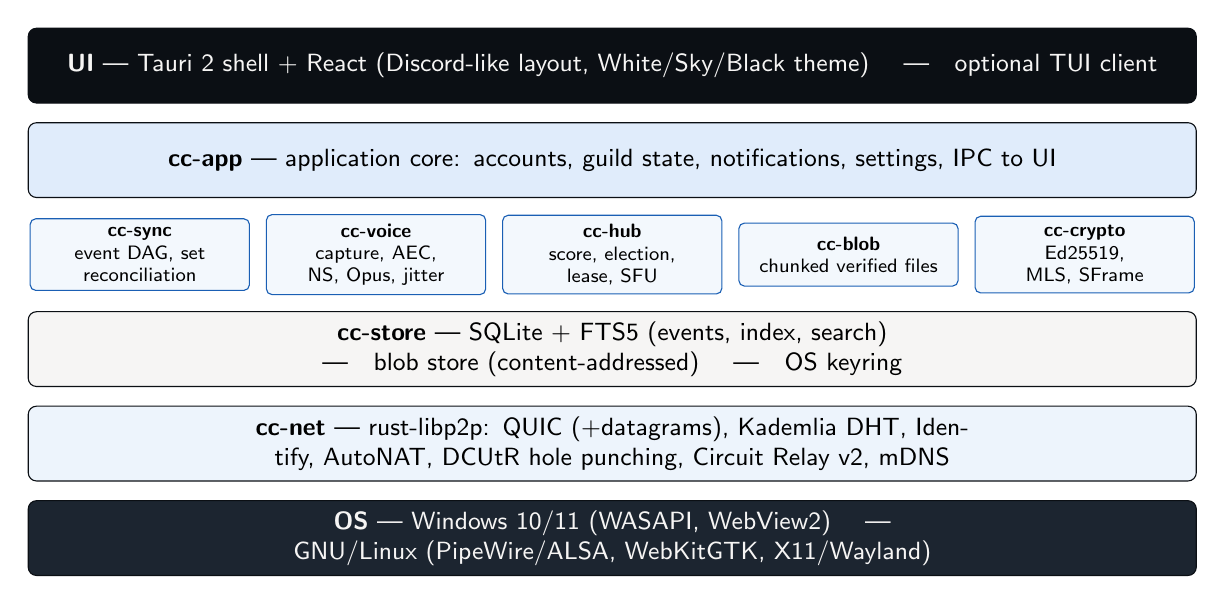
\begin{tikzpicture}[
  layer/.style={draw=ccblack,fill=#1,rounded corners=3pt,minimum height=0.95cm,
                text width=14.6cm,align=center,font=\sffamily\small},
  mod/.style={draw=ccskyd,fill=ccsky!12,rounded corners=2pt,minimum height=0.8cm,
              text width=2.55cm,align=center,font=\sffamily\scriptsize}]
  \node[layer=ccblack,text=ccwhite] (ui) at (0,6.2) {\textbf{UI} --- Tauri 2 shell + React (Discord-like layout, White/Sky/Black theme) \quad|\quad optional TUI client};
  \node[layer=ccsky!30] (core) at (0,5.0) {\textbf{cc-app} --- application core: accounts, guild state, notifications, settings, IPC to UI};
  \node[mod] (m1) at (-6.0,3.8) {\textbf{cc-sync}\\event DAG, set reconciliation};
  \node[mod] (m2) at (-3.0,3.8) {\textbf{cc-voice}\\capture, AEC, NS, Opus, jitter};
  \node[mod] (m3) at (0,3.8)    {\textbf{cc-hub}\\score, election, lease, SFU};
  \node[mod] (m4) at (3.0,3.8)  {\textbf{cc-blob}\\chunked verified files};
  \node[mod] (m5) at (6.0,3.8)  {\textbf{cc-crypto}\\Ed25519, MLS, SFrame};
  \node[layer=ccwhite] (store) at (0,2.6) {\textbf{cc-store} --- SQLite + FTS5 (events, index, search) \quad|\quad blob store (content-addressed) \quad|\quad OS keyring};
  \node[layer=ccsky!18] (net) at (0,1.4) {\textbf{cc-net} --- rust-libp2p: QUIC (+datagrams), Kademlia DHT, Identify, AutoNAT, DCUtR hole punching, Circuit Relay v2, mDNS};
  \node[layer=ccpanel2,text=ccwhite] (os) at (0,0.2) {\textbf{OS} --- Windows 10/11 (WASAPI, WebView2) \quad|\quad GNU/Linux (PipeWire/ALSA, WebKitGTK, X11/Wayland)};
\end{tikzpicture}
\caption{Layered architecture of a CyberCord peer. Every peer runs the full stack; there is
no separate ``server build'' --- a Keeper is the same core without the UI. All crates share
\texttt{cc-proto} (types and wire format).}
\label{fig:arch}
\end{figure}

% =====================================================================
\section{The \SCOOP/1 protocol}
% =====================================================================

\subsection{Identity}
\begin{itemize}
  \item \textbf{Root identity key} (Ed25519) generated on first start; backed up as a
        24-word recovery phrase. Stored encrypted in the OS keyring.
  \item \textbf{Device keys} signed by the root key (\texttt{DeviceCert}), so one person can
        run CyberCord on a desktop and a laptop. Revocation is an event.
  \item \textbf{Network PeerId} = the libp2p identity of the device key; QUIC/TLS 1.3
        handshakes prove it, so a connection cannot be impersonated.
  \item \textbf{Display name and avatar} are profile events signed by the root key and
        replicated like any other data.
\end{itemize}

\subsection{Transport and NAT traversal}
\begin{itemize}
  \item \textbf{QUIC over UDP} for everything: reliable streams for events and files,
        unreliable \textbf{QUIC datagrams} (RFC 9221) for voice.
  \item \textbf{AutoNAT} classifies each peer's reachability (public, full-cone,
        restricted, symmetric).
  \item \textbf{DCUtR} performs coordinated UDP hole punching through a peer both sides
        already know.
  \item \textbf{Circuit Relay v2}: when punching fails, any public peer that opted in
        (often the hub or a Keeper) relays the traffic. Relays see only encrypted bytes.
  \item \textbf{One UDP port} per peer (default 47100, random fallback); Windows installer
        adds a firewall rule; on Linux the port is shown in settings.
\end{itemize}

\subsection{Discovery and bootstrap}
A new peer must reach \emph{at least one} other peer once; after that it never needs a
server again. It tries these sources in order, cheapest first:

\begin{enumerate}
  \item \textbf{Session cache} --- signed addresses of peers it talked to last time.
  \item \textbf{Local network} --- \textbf{mDNS}, plus an optional bounded sweep of the
        peer's \emph{own} subnet (e.g.\ the local \texttt{/24}) on the CyberCord port.
        This finds people on the same Wi-Fi, LAN party or office with no internet at all.
  \item \textbf{Invite link or QR code} --- carries the guild id, a token and a few current
        peer addresses (format below).
  \item \textbf{Kademlia DHT} --- once any peer is reached, the client joins the DHT and
        looks up users, guild providers and public directory records:
  \begin{itemize}
    \item \texttt{H("peer"\,||\,user\_id)} $\to$ current signed address record of a user;
    \item \texttt{H("guild"\,||\,guild\_id)} $\to$ peers online in a guild (\emph{providers});
    \item \texttt{H("dir"\,||\,tag)} $\to$ signed public directory listings for discovery.
  \end{itemize}
  \item \textbf{Community bootstrap peers} --- a signed, replaceable seed list
        (SocioCyberneering Keepers and volunteer peers). Any peer can be a seed, none is
        required, and the list is updated through a guild event rather than hard-coded.
\end{enumerate}

\noindent Invite link format:
\begin{lstlisting}[language={},numbers=none]
cybercord://join/<guild_id_base32>?t=<invite_token>&a=<multiaddr_1>,<multiaddr_2>
\end{lstlisting}

% ---------------------------------------------------------------------
\subsection{Finding users without servers: gossip and the peer address book}
\label{sec:pex}

Once a peer knows even one other peer, the network grows by itself through
\textbf{peer exchange} (PEX / gossip): on every connection the two sides trade the signed
address records they already hold. One contact becomes dozens within seconds, and dozens
become the whole reachable network --- with no central directory and without probing
strangers.

\begin{figure}[ht]
\centering
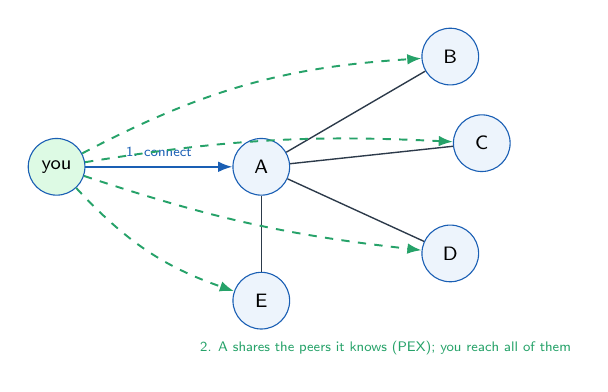
\begin{tikzpicture}[
  peer/.style={circle,draw=ccskyd,fill=ccsky!18,minimum size=0.72cm,inner sep=0,font=\sffamily\scriptsize},
  known/.style={-{Latex[length=1.8mm]},ccskyd,line width=0.7pt},
  learn/.style={-{Latex[length=1.8mm]},ccgreend,line width=0.7pt,dashed}]
  \node[peer,fill=ccgreen!30] (you) at (0,0) {you};
  \node[peer] (a) at (2.6,0) {A};
  \node[peer] (b) at (5.0,1.4) {B};
  \node[peer] (c) at (5.4,0.3) {C};
  \node[peer] (d) at (5.0,-1.1) {D};
  \node[peer] (e) at (2.6,-1.7) {E};
  \draw[known] (you)--(a) node[midway,above,font=\sffamily\tiny,text=ccskyd] {1. connect};
  \draw[ccline,line width=0.5pt] (a)--(b); \draw[ccline,line width=0.5pt] (a)--(c);
  \draw[ccline,line width=0.5pt] (a)--(d); \draw[ccline,line width=0.5pt] (a)--(e);
  \draw[learn] (you) to[bend left=12] (b);
  \draw[learn] (you) to[bend left=6] (c);
  \draw[learn] (you) to[bend right=6] (d);
  \draw[learn] (you) to[bend right=14] (e);
  \node[font=\sffamily\tiny,text=ccgreend,anchor=west] at (1.7,-2.3) {2. A shares the peers it knows (PEX); you reach all of them};
\end{tikzpicture}
\caption{Peer exchange. Reaching one peer (A) yields A's whole address book; the list
grows outward with no central server and no scanning.}
\label{fig:pex}
\end{figure}

\paragraph{Peer address book (the ``users list'').} Each client keeps a local, signed
table of the peers it has learned about --- effectively the app's offline ``who is out
there'' list:

\begin{center}\small
\begin{tabularx}{\linewidth}{@{}l Y@{}}
\toprule
\textbf{Field} & \textbf{Meaning} \\
\midrule
\texttt{user\_id} & BLAKE3 of the peer's public key \\
\texttt{addresses} & last-known multiaddrs (direct, relayed) \\
\texttt{nat} & reachability class (public / full-cone / restricted / symmetric) \\
\texttt{last\_seen} & when the peer was last reached \\
\texttt{rtt\_ms} & measured latency, for nearest-first ordering \\
\texttt{source} & how it was learned: LAN / invite / DHT / PEX \\
\bottomrule
\end{tabularx}
\end{center}

\noindent The book is private to the device, never uploaded, and holds only peers that
\emph{advertised themselves} (through the DHT, an invite or gossip) --- never addresses
harvested by scanning. It is the honest version of a ``list of users' IPs''.

\paragraph{Finding nearby users first.} To connect fast, the client prefers low-latency,
same-region peers: DHT and PEX results are ordered by measured RTT and by shared guilds,
so people close to you (usually in your country) are tried first. This gives the
``find nearby users quickly'' behaviour \emph{without} scanning any address space.

\paragraph{Bounded probing only.} NAT hole-punching does send a few small UDP packets, but
only to a \emph{specific candidate} already learned from the LAN, an invite, the DHT or
gossip, and it is rate-limited. CyberCord never sprays probe packets at addresses that did
not announce themselves.

\begin{honest}[Why CyberCord does not scan the internet for users]
Mass-scanning IP ranges and flooding ``discovery'' packets is tempting when there are no
servers, but it is the wrong tool and it backfires on the very goal of staying unblockable:
\begin{itemize}[leftmargin=1.2em]
  \item \textbf{It gets \emph{your} machine blocked.} ISPs, firewalls and abuse systems
        flag a host that sends unsolicited packets to many addresses; the scanner's own IP
        is rate-limited, null-routed and reported --- exactly the ``being blocked'' outcome
        a serverless design exists to avoid.
  \item \textbf{It does not scale.} IPv4 is $\approx$4.3 billion addresses --- weeks of
        flooding from a home link --- and IPv6, which most users now get, is far too large
        to sweep at all.
  \item \textbf{Most users have no address to scan.} Behind NAT there is no public address;
        such peers are reachable only by rendezvous (DHT / PEX / relay), which CyberCord
        already uses.
  \item \textbf{Gossip is simply faster.} PEX reaches the active network in seconds;
        scanning would take days to find the same people.
\end{itemize}
Same goal, correct mechanism: \textbf{gossip + DHT + LAN + invites}, ordered nearest-first,
with bounded probing of candidates that announced themselves.
\end{honest}

% ---------------------------------------------------------------------
\subsection{Adaptive topology ladder: $p2p \to p3p \to \dots \to pNp$}
\label{sec:ladder}

The number of active peers $N$ in a room decides how they connect. Small rooms use a
\emph{full mesh} (everybody talks to everybody --- the lowest latency). Larger rooms
switch to a \emph{star} around the elected Virtual Hub. Very large rooms use a
\emph{cascade} of hubs.

\begin{figure}[ht]
\centering
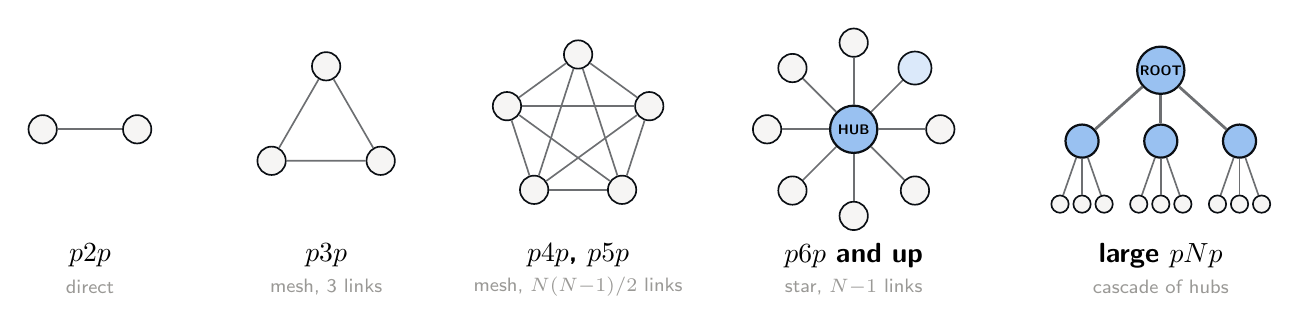
\begin{tikzpicture}[
  pe/.style={circle,fill=ccwhite,draw=ccblack,line width=0.6pt,inner sep=0pt,minimum size=0.36cm},
  hub/.style={circle,fill=ccsky,draw=ccblack,line width=0.8pt,inner sep=0pt,minimum size=0.6cm,font=\tiny\sffamily\bfseries},
  ln/.style={ccblack!60,line width=0.6pt}]
  % p2p
  \begin{scope}[shift={(0,0)}]
    \node[pe] (a) at (-0.6,0) {}; \node[pe] (b) at (0.6,0) {};
    \draw[ln] (a)--(b);
    \node[font=\sffamily\bfseries] at (0,-1.6) {$p2p$};
    \node[font=\sffamily\scriptsize,color=ccgray] at (0,-2.0) {direct};
  \end{scope}
  % p3p
  \begin{scope}[shift={(3.0,0)}]
    \foreach \i in {1,2,3}{\node[pe] (n\i) at (90+\i*120:0.8) {};}
    \draw[ln] (n1)--(n2)--(n3)--(n1);
    \node[font=\sffamily\bfseries] at (0,-1.6) {$p3p$};
    \node[font=\sffamily\scriptsize,color=ccgray] at (0,-2.0) {mesh, 3 links};
  \end{scope}
  % p5p
  \begin{scope}[shift={(6.2,0)}]
    \foreach \i in {1,...,5}{\node[pe] (q\i) at (90+\i*72:0.95) {};}
    \foreach \i in {1,...,5}{\foreach \j in {1,...,5}{\ifnum\i<\j \draw[ln] (q\i)--(q\j);\fi}}
    \node[font=\sffamily\bfseries] at (0,-1.6) {$p4p$, $p5p$};
    \node[font=\sffamily\scriptsize,color=ccgray] at (0,-2.0) {mesh, $N(N{-}1)/2$ links};
  \end{scope}
  % p6p+
  \begin{scope}[shift={(9.7,0)}]
    \node[hub] (h) at (0,0) {HUB};
    \foreach \i in {1,...,8}{\node[pe] (s\i) at (\i*45:1.1) {}; \draw[ln] (h)--(s\i);}
    \node[pe,fill=ccsky!35,minimum size=0.42cm] at (45:1.1) {};
    \node[font=\sffamily\bfseries] at (0,-1.6) {$p6p$ and up};
    \node[font=\sffamily\scriptsize,color=ccgray] at (0,-2.0) {star, $N{-}1$ links};
  \end{scope}
  % cascade
  \begin{scope}[shift={(13.6,0)}]
    \node[hub] (r) at (0,0.75) {ROOT};
    \foreach \k/\x in {1/-1.0,2/0,3/1.0}{
      \node[hub,minimum size=0.42cm,font=\tiny] (c\k) at (\x,-0.15) {};
      \draw[ln,line width=1pt] (r)--(c\k);
      \foreach \m/\dx in {1/-0.28,2/0,3/0.28}{\node[pe,minimum size=0.22cm] (l\k\m) at (\x+\dx,-0.95) {}; \draw[ln] (c\k)--(l\k\m);}
    }
    \node[font=\sffamily\bfseries] at (0,-1.6) {large $pNp$};
    \node[font=\sffamily\scriptsize,color=ccgray] at (0,-2.0) {cascade of hubs};
  \end{scope}
\end{tikzpicture}
\caption{Topology ladder. Light blue peer in the star = Standby. The level is
re-evaluated whenever someone joins or leaves.}
\label{fig:ladder}
\end{figure}

\paragraph{Bandwidth model.} Let $b$ be the on-wire bitrate of one voice stream. With
Opus at 32\,kbit/s, 20\,ms frames (50 packets/s) and roughly 70 bytes of IP/UDP/QUIC/\SCOOP{}
overhead per packet, $b \approx 32 + 50\cdot 70\cdot 8/1000 \approx 60$\,kbit/s. Let $S$ be the
maximum number of simultaneous speakers forwarded to each listener (default $S=3$, the
loudest three).

\begin{align}
\text{Mesh:}\quad & U_{\text{peer}} = D_{\text{peer}} = (N-1)\,b \\
\text{Star:}\quad & U_{\text{peer}} = b, \qquad D_{\text{peer}} = \min(S, N-1)\,b, \qquad
                    U_{\text{hub}} \approx (N-1)\,\min(S, N-1)\,b
\end{align}

The room leaves mesh mode when either $N \ge N_{\text{mesh}}$ (default 6) or the weakest
peer cannot carry the mesh:
\begin{equation}
  (N-1)\,b \;>\; \alpha \, U_{\min}, \qquad \alpha = 0.5 .
\end{equation}
One hub serves at most $C = \lfloor \alpha\,U_{\text{hub}} / (S\,b) \rfloor$ listeners; beyond
that the hub becomes the \emph{root} of a cascade and delegates to sub-hubs.

\begin{table}[ht]
\centering
\small
\begin{tabular}{@{}lrlrr@{}}
\toprule
\textbf{Level} & $N$ & \textbf{Topology} & \textbf{Peer uplink} & \textbf{Hub uplink} \\
\midrule
$p2p$ & 2 & direct          & 60 kbit/s  & --- \\
$p3p$ & 3 & mesh            & 120 kbit/s & --- \\
$p4p$ & 4 & mesh            & 180 kbit/s & --- \\
$p5p$ & 5 & mesh            & 240 kbit/s & --- \\
$p6p$ & 6 & star (hub)      & 60 kbit/s  & 0.90 Mbit/s \\
$p10p$ & 10 & star          & 60 kbit/s  & 1.62 Mbit/s \\
$p50p$ & 50 & star          & 60 kbit/s  & 8.82 Mbit/s \\
$p200p$ & 200 & cascade (root + 2 sub-hubs) & 60 kbit/s & $\approx$18 Mbit/s per sub-hub \\
\bottomrule
\end{tabular}
\caption{Voice bandwidth by level ($b = 60$\,kbit/s, $S = 3$). With a 50\,Mbit/s hub uplink
and $\alpha=0.6$, one hub carries $C = \lfloor 30000/180 \rfloor = 166$ listeners, so 200
peers need a cascade. With DTX and voice activity detection, silent peers send almost nothing.}
\label{tab:bw}
\end{table}

Text-only rooms use the same ladder, but the numbers are tiny; there the hub mainly
gives fast fan-out and a single place for newcomers to sync from.

% ---------------------------------------------------------------------
\subsection{Virtual Hub election}
\label{sec:election}

\subsubsection{Hub score}
Every peer continuously measures itself and gossips a signed \texttt{SCORE} record to the
room every 5\,s. The score $S_i \in [0,1]$ is:

\begin{equation}
S_i \;=\; V_i \cdot \big( w_b B_i + w_c C_i + w_n R_i + w_u T_i + w_p P_i \big)
\label{eq:score}
\end{equation}

\begin{center}
\small
\begin{tabularx}{\linewidth}{@{}l l Y r@{}}
\toprule
\textbf{Term} & \textbf{Meaning} & \textbf{Definition} & \textbf{Weight} \\
\midrule
$B_i$ & upload capacity & $\min\!\big(1,\ \log(1 + U_i/1\,\text{Mbit/s}) / \log 101\big)$ --- 100\,Mbit/s $\to$ 1 & $w_b = 0.35$ \\
$C_i$ & centrality & $1 - \tilde{r}_i / 300\,\text{ms}$, where $\tilde{r}_i$ = median RTT from $i$ to room members (clamped) & $w_c = 0.25$ \\
$R_i$ & reachability & public 1.0 $\cdot$ full-cone 0.8 $\cdot$ restricted 0.5 $\cdot$ symmetric 0.1 & $w_n = 0.20$ \\
$T_i$ & stability & $\min(1,\ t_{\text{online}} / 30\,\text{min})$ & $w_u = 0.10$ \\
$P_i$ & power & desktop / AC 1.0 $\cdot$ laptop on battery 0.3 & $w_p = 0.10$ \\
$V_i$ & veto & 0 if the user chose \emph{never host}, connection is metered, CPU $>$ 85\%, or Shielded mode; else 1 & --- \\
\bottomrule
\end{tabularx}
\end{center}

$U_i$ is estimated passively from the QUIC congestion controller and occasionally refined
with a short probe. To spread load, the effective score is $\hat{S}_i = S_i\,(1 - L_i)$,
where $L_i$ is the share of the peer's capacity already used hosting other rooms.

\subsubsection{Deterministic election}
Every peer runs the same function on the same gossiped table, so they all reach the same
result without voting rounds.

\begin{algorithm}[ht]
\caption{Virtual Hub election for channel $c$ (run identically on every peer)}
\label{alg:elect}
\KwIn{score table $\mathcal{T}=\{(p, S_p, L_p, t_p)\}$ from \texttt{SCORE} gossip; current lease $(e, h)$; hysteresis $\eta = 0.2$}
\KwOut{hub $h^\ast$, standby $s^\ast$, epoch $e'$}
$\mathcal{C} \gets \{\,p \in \mathcal{T} : S_p > 0 \text{ and } t_p \text{ younger than } 15\,\text{s}\,\}$\;
\ForEach{$p \in \mathcal{C}$}{ $\hat{S}_p \gets S_p\,(1 - L_p)$\; }
sort $\mathcal{C}$ by $\hat{S}_p$ descending; break ties by $\mathrm{BLAKE3}(p \,\|\, c \,\|\, e)$ ascending\;
$h^\ast \gets \mathcal{C}[0]$;\quad $s^\ast \gets \mathcal{C}[1]$\;
\eIf{lease $(e,h)$ is alive \textbf{and} $h \in \mathcal{C}$ \textbf{and} $\hat{S}_{h^\ast} < (1+\eta)\,\hat{S}_h$}{
  \Return{$(h,\ s^\ast,\ e)$} \tcp*{keep current hub (no flapping)}
}{
  \Return{$(h^\ast,\ s^\ast,\ e+1)$} \tcp*{hand over to a clearly better peer}
}
\end{algorithm}

The winner announces a signed \texttt{LEASE\{channel, epoch, hub, standby, expires\}}.
Peers accept a lease if it agrees with their own computation (small differences in score
tables are tolerated: a lease is accepted if its hub is in the local top three).

\subsubsection{Lease, heartbeat and failover}
\begin{itemize}
  \item The hub sends \texttt{HEARTBEAT} every \textbf{500\,ms}; a lease lasts \textbf{2\,s}.
  \item All peers keep an idle, already-authenticated QUIC connection to the
        \textbf{standby} (a \emph{warm} path), so failover needs no new handshakes.
  \item \textbf{Graceful handover:} when the hub user closes the app or their score drops,
        the hub sends \texttt{YIELD}; the standby takes over immediately --- no audible gap.
  \item \textbf{Crash failover:} if no heartbeat arrives before the lease expires, the
        standby issues a new \texttt{LEASE} with epoch $e{+}1$; peers move their streams. Expected audio
        gap: about 1--2\,s, covered by packet-loss concealment.
  \item \textbf{Split brain:} if the network splits, each half elects its own hub. On merge,
        the lease with the higher (epoch, score, $-$hash) wins and the other hub demotes
        itself. Chat history merges automatically because it is a DAG (\S\ref{sec:dag}).
\end{itemize}

\begin{figure}[ht]
\centering
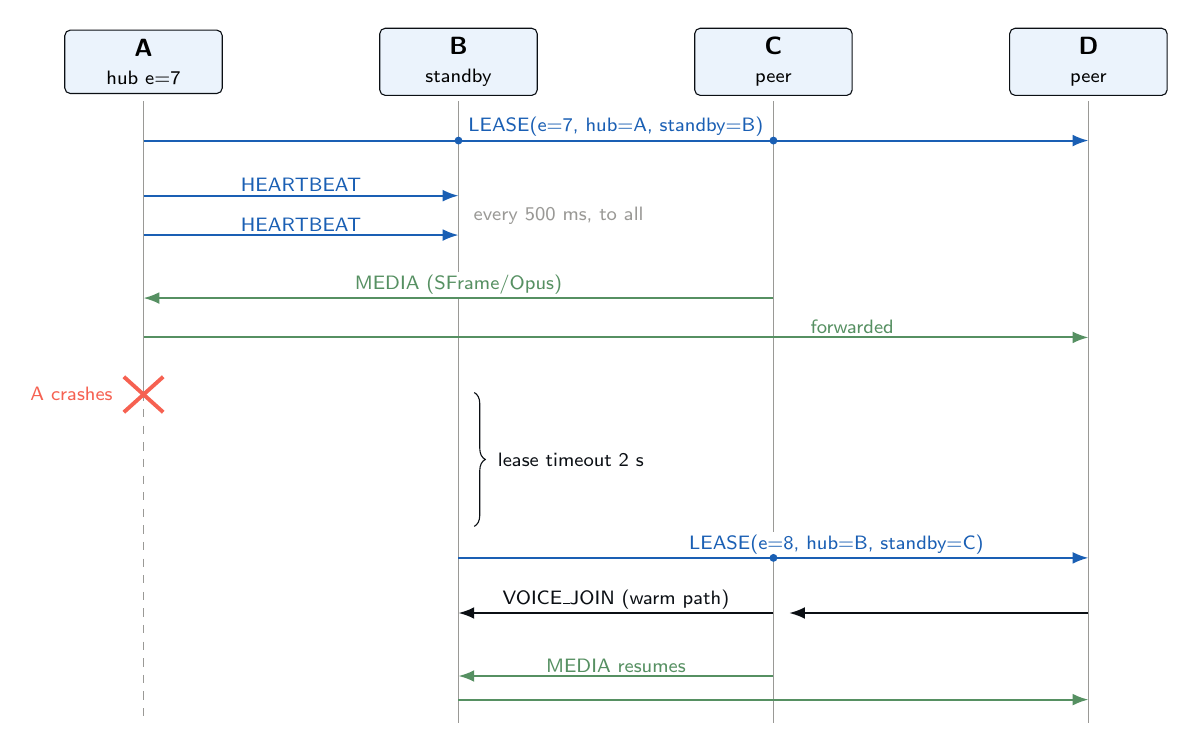
\begin{tikzpicture}[
  msg/.style={-{Latex[length=2mm]},line width=0.7pt,ccskyd},
  lbl/.style={font=\sffamily\scriptsize,fill=white,inner sep=1pt}]
  \foreach \x/\n/\r in {0/A/hub e=7,4/B/standby,8/C/peer,12/D/peer}{
    \node[draw=ccblack,fill=ccsky!20,rounded corners=2pt,font=\sffamily\small,minimum width=2cm,align=center] at (\x,0) {\textbf{\n}\\[-1pt]{\scriptsize \r}};
  }
  \draw[ccgray,line width=0.6pt] (0,-0.5) -- (0,-4.2);
  \draw[ccgray,dashed] (0,-4.2) -- (0,-8.4);
  \foreach \x in {4,8,12}{\draw[ccgray,line width=0.6pt] (\x,-0.5) -- (\x,-8.4);}
  \draw[msg] (0,-1.0) -- (12,-1.0) node[lbl,midway,above] {LEASE(e=7, hub=A, standby=B)};
  \fill[ccskyd] (4,-1.0) circle (0.05); \fill[ccskyd] (8,-1.0) circle (0.05);
  \draw[msg] (0,-1.7) -- (4,-1.7) node[lbl,midway,above] {HEARTBEAT};
  \draw[msg] (0,-2.2) -- (4,-2.2) node[lbl,midway,above] {HEARTBEAT};
  \node[lbl,anchor=west,text=ccgray] at (4.15,-1.95) {every 500 ms, to all};
  \draw[msg,ccgreen!60!black] (8,-3.0) -- (0,-3.0) node[lbl,pos=0.5,above] {MEDIA (SFrame/Opus)};
  \draw[msg,ccgreen!60!black] (0,-3.5) -- (12,-3.5) node[lbl,pos=0.75,above] {forwarded};
  \draw[ccred,line width=1.4pt] (-0.25,-4.0) -- (0.25,-4.45) (-0.25,-4.45) -- (0.25,-4.0);
  \node[lbl,anchor=east,text=ccred] at (-0.35,-4.22) {A crashes};
  \draw[decorate,decoration={brace,amplitude=4pt},ccblack] (4.2,-4.2) -- (4.2,-5.9) node[midway,right=5pt,font=\sffamily\scriptsize] {lease timeout 2 s};
  \draw[msg] (4,-6.3) -- (12,-6.3) node[lbl,pos=0.6,above] {LEASE(e=8, hub=B, standby=C)};
  \fill[ccskyd] (8,-6.3) circle (0.05);
  \draw[msg,ccblack] (8,-7.0) -- (4,-7.0) node[lbl,midway,above] {VOICE\_JOIN (warm path)};
  \draw[msg,ccblack] (12,-7.0) -- (8.2,-7.0);
  \draw[msg,ccgreen!60!black] (8,-7.8) -- (4,-7.8) node[lbl,midway,above] {MEDIA resumes};
  \draw[msg,ccgreen!60!black] (4,-8.1) -- (12,-8.1);
\end{tikzpicture}
\caption{Crash failover. The standby already holds warm connections, so the switch is
a single signed lease plus re-subscription.}
\label{fig:failover}
\end{figure}

\subsubsection{Why an untrusted hub is safe}
The hub can only \emph{forward} or \emph{drop}. It cannot forge messages (every event is
signed), cannot read private content (MLS for text, SFrame for media), and cannot rewrite
history (event IDs are hashes over their parents). Peers detect a hub that silently
drops traffic by comparing receipt digests on the standby path; a suspicious hub gets
a local penalty $V_i = 0$ for that room and the election moves on.

% ---------------------------------------------------------------------
\subsection{Event graph and synchronisation}
\label{sec:dag}

All guild data --- messages, edits, reactions, channel and role changes --- are
\textbf{events}. Each event is signed and points to the latest events its author had seen
(its \emph{parents}). The result is a directed acyclic graph (DAG) that behaves like a CRDT:
two peers holding the same set of events always compute the same state, no matter the
order in which events arrived.

\begin{figure}[ht]
\centering
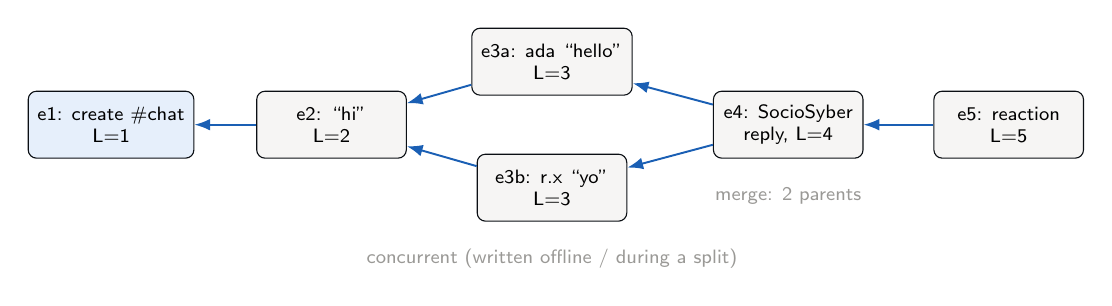
\begin{tikzpicture}[
  ev/.style={draw=ccblack,fill=ccwhite,rounded corners=3pt,font=\sffamily\scriptsize,align=center,minimum width=1.9cm,minimum height=0.85cm},
  ref/.style={-{Latex[length=2mm]},ccskyd,line width=0.7pt}]
  \node[ev,fill=ccsky!25] (e1) at (0,0)    {e1: create \#chat\\ L=1};
  \node[ev] (e2) at (2.8,0)  {e2: ``hi''\\ L=2};
  \node[ev] (e3) at (5.6,0.8) {e3a: ada ``hello''\\ L=3};
  \node[ev] (e4) at (5.6,-0.8){e3b: r.x ``yo''\\ L=3};
  \node[ev] (e5) at (8.6,0)  {e4: SocioSyber\\ reply, L=4};
  \node[ev] (e6) at (11.4,0) {e5: reaction\\ L=5};
  \draw[ref] (e2)--(e1); \draw[ref] (e3)--(e2); \draw[ref] (e4)--(e2);
  \draw[ref] (e5)--(e3); \draw[ref] (e5)--(e4); \draw[ref] (e6)--(e5);
  \node[font=\sffamily\scriptsize,color=ccgray] at (5.6,-1.7) {concurrent (written offline / during a split)};
  \node[font=\sffamily\scriptsize,color=ccgray] at (8.6,-0.9) {merge: 2 parents};
\end{tikzpicture}
\caption{Event DAG. Arrows point to parents. Display order is by Lamport clock $L$, then
wall time, then event ID --- identical on every peer.}
\label{fig:dag}
\end{figure}

\begin{itemize}
  \item \textbf{Event ID} = BLAKE3 over the canonical encoding (postcard) of the signed event.
  \item \textbf{Live delivery:} in hub mode, the author sends the event to the hub, which
        fans it out; in mesh mode, peers send it to each other directly.
  \item \textbf{Catch-up:} on connect, peers exchange channel \emph{heads}. If they differ,
        they run \textbf{range-based set reconciliation} over event IDs in time windows:
        cost grows with the \emph{difference}, not with the history size.
  \item \textbf{Validation:} each received event is checked for signature, parents present,
        and permission (\S\ref{sec:perm}) before it is stored or forwarded.
  \item \textbf{Offline DMs:} the sender's client and any Keeper the two users share hold an
        encrypted \emph{mailbox} copy until the recipient comes online.
\end{itemize}

% ---------------------------------------------------------------------
\subsection{Local storage and files}
\label{sec:storage}

Everything is stored on the user's PC:
\begin{itemize}
  \item \textbf{Events and search:} SQLite with an FTS5 full-text index;
        database encrypted with a key held in the OS keyring
        (Windows Credential Manager, Linux Secret Service; passphrase fallback for
        minimal desktops without a keyring daemon).
  \item \textbf{Files (blobs):} split into chunks, hashed as a BLAKE3 tree, so every chunk
        is verified as it arrives and a download can pull chunks from many members at once
        (swarming, like BitTorrent). A message only carries the root hash, size, MIME type
        and --- for private channels --- the decryption key.
\end{itemize}

\paragraph{Relation to IPFS.} This blob layer is content-addressed and swarmed, which is
exactly the IPFS model, so CyberCord can adopt the IPFS stack rather than reinvent it.
Two practical options:
\begin{itemize}
  \item \textbf{IPFS-style, embedded (recommended):} use \texttt{iroh} --- a Rust,
        QUIC-native content-addressed transfer library in the IPFS family. It reuses the
        peer connections CyberCord already has, keeps content private by default, and needs
        no separate daemon.
  \item \textbf{Full IPFS:} run against a \texttt{kubo}/\texttt{rust-ipfs} node and publish
        blobs by CID. This buys interop with the public IPFS network, at the cost of a
        heavier dependency and more metadata exposure (the public IPFS DHT reveals who
        requests which CID), so private channels would still wrap content in their own key.
\end{itemize}

\begin{honest}[IPFS does not make offline files appear]
Content addressing lets \emph{any} holder serve a file and guarantees integrity, but a file
is downloadable only while \emph{someone who has it is online} --- IPFS has no magic offline
store. Availability when the author is offline comes from \textbf{pinning}: the
``Keeper'' and ``Full'' policies below pin blobs on always-on machines (a home server,
Orange~Pi or VPS), and popular files are naturally cached by many members. This is the same
limitation, and the same fix, whether the layer is plain BLAKE3 swarming, \texttt{iroh}, or
full IPFS.
\end{honest}

\begin{center}
\small
\begin{tabularx}{\linewidth}{@{}l Y@{}}
\toprule
\textbf{Storage policy (per guild)} & \textbf{Behaviour} \\
\midrule
Keeper & Full history and all files, pinned forever, serves everyone. For always-on machines. \\
Full   & Full text history; files cached up to a quota. \\
Recent (default) & Last 90 days of text, 500\,MB media cache; older data fetched on demand. \\
Light  & Metadata and own messages only; everything else on demand. \\
\bottomrule
\end{tabularx}
\end{center}

% ---------------------------------------------------------------------
\subsection{Encryption}
\label{sec:crypto}

\begin{center}
\small
\begin{tabularx}{\linewidth}{@{}l Y@{}}
\toprule
\textbf{Layer} & \textbf{Mechanism} \\
\midrule
Transport & QUIC with TLS 1.3, peer identity bound to the certificate (all traffic, always). \\
Authenticity & Ed25519 signature on every event and lease. \\
DMs, group DMs, private channels & \textbf{MLS} (RFC 9420): group keys with forward secrecy and post-compromise security; efficient for large groups. \\
Voice/video in private rooms & \textbf{SFrame} (RFC 9605): media frames encrypted end-to-end with keys derived from the MLS group; the hub forwards ciphertext. \\
Public community channels & Signed but not end-to-end encrypted (anyone may join and read); encrypted in transit and at rest. \\
At rest & Local database and blob store encrypted; key in OS keyring. \\
\bottomrule
\end{tabularx}
\end{center}

\noindent For loudest-speaker selection, each media packet carries a 1-byte audio level in
the clear header. This tells the hub \emph{when} someone speaks, but not \emph{what} they say.

% ---------------------------------------------------------------------
\subsection{Permissions and moderation without a server}
\label{sec:perm}

\begin{itemize}
  \item A guild starts with a signed \textbf{genesis event} by its owner. Roles, permission
        changes, bans and channel edits are events signed by someone who holds the right
        permission \emph{in the state defined by that event's parents}.
  \item Every peer applies the same deterministic \textbf{authorization rules}; an event that
        fails them is not stored and not forwarded. There is no server to bypass.
  \item Concurrent conflicts (e.g.\ an admin is demoted while banning someone) are resolved
        by power level, then Lamport clock, then event ID.
  \item \textbf{Owner safety:} owner rights can be a 2-of-3 threshold of admin keys, so a lost
        key does not orphan a guild.
  \item \textbf{Anti-spam:} join requires an invite token or a proof-of-work stamp (difficulty
        set per guild); every peer enforces per-author rate limits and drops floods instead of
        relaying them.
\end{itemize}

% ---------------------------------------------------------------------
\subsection{Wire messages}

All frames are \texttt{postcard}-encoded Rust enums over the libp2p protocol
\texttt{/cybercord/scoop/1}. Media uses QUIC datagrams.

\begin{center}
\small
\begin{tabularx}{\linewidth}{@{}l l Y@{}}
\toprule
\textbf{Frame} & \textbf{Channel} & \textbf{Purpose} \\
\midrule
\texttt{HELLO}       & stream & version, capabilities, device certificate \\
\texttt{PING/PONG}   & stream & RTT measurement for centrality \\
\texttt{SCORE}       & stream & signed hub-score record (every 5\,s) \\
\texttt{LEASE}       & stream & signed hub/standby assignment with epoch and expiry \\
\texttt{HEARTBEAT}   & stream & lease renewal, every 500\,ms \\
\texttt{YIELD}       & stream & graceful hub hand-over \\
\texttt{HEADS}       & stream & current DAG heads of a channel \\
\texttt{RECON}       & stream & one round of range-based set reconciliation \\
\texttt{EVENTS}      & stream & batch of signed events \\
\texttt{BLOB\_GET/PART} & stream & request / deliver verified file chunks \\
\texttt{VOICE\_JOIN/LEAVE} & stream & enter or leave a voice room \\
\texttt{SUBSCRIBE}   & stream & which speakers/streams a listener wants \\
\texttt{PRESENCE}    & stream & online / idle / do-not-disturb, typing \\
\texttt{MAILBOX\_PUT/GET} & stream & store-and-forward for offline DMs \\
\texttt{MEDIA}       & datagram & header (room id, stream id, seq, timestamp, level, flags) + SFrame(Opus) \\
\bottomrule
\end{tabularx}
\end{center}

% =====================================================================
\section{Voice and noise suppression}
\label{sec:voice}
% =====================================================================

\begin{figure}[ht]
\centering
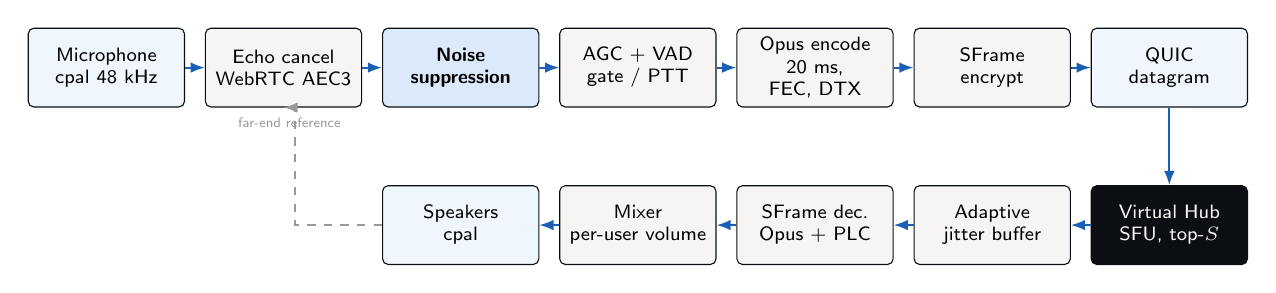
\begin{tikzpicture}[
  st/.style={draw=ccblack,fill=#1,rounded corners=2pt,font=\sffamily\scriptsize,align=center,minimum height=1.0cm,text width=1.75cm},
  st/.default=ccwhite,
  ar/.style={-{Latex[length=1.8mm]},line width=0.7pt,ccskyd}]
  \node[st=ccsky!15] (mic) at (0,0) {Microphone\\cpal 48 kHz};
  \node[st] (aec) at (2.25,0) {Echo cancel\\WebRTC AEC3};
  \node[st=ccsky!35] (ns) at (4.5,0) {\textbf{Noise\\suppression}};
  \node[st] (agc) at (6.75,0) {AGC + VAD\\gate / PTT};
  \node[st] (enc) at (9.0,0) {Opus encode\\20 ms, FEC, DTX};
  \node[st] (sf) at (11.25,0) {SFrame\\encrypt};
  \node[st=ccsky!15] (q) at (13.5,0) {QUIC\\datagram};
  \node[st=ccblack,text=ccwhite] (hub) at (13.5,-2.0) {Virtual Hub\\SFU, top-$S$};
  \node[st] (jb) at (11.25,-2.0) {Adaptive\\jitter buffer};
  \node[st] (dec) at (9.0,-2.0) {SFrame dec.\\Opus + PLC};
  \node[st] (mix) at (6.75,-2.0) {Mixer\\per-user volume};
  \node[st=ccsky!15] (out) at (4.5,-2.0) {Speakers\\cpal};
  \draw[ar] (mic)--(aec); \draw[ar] (aec)--(ns); \draw[ar] (ns)--(agc); \draw[ar] (agc)--(enc);
  \draw[ar] (enc)--(sf); \draw[ar] (sf)--(q); \draw[ar] (q)--(hub); \draw[ar] (hub)--(jb);
  \draw[ar] (jb)--(dec); \draw[ar] (dec)--(mix); \draw[ar] (mix)--(out);
  \draw[ar,dashed,ccgray] (out.west) -| ++(-1.1,1.0) |- (aec.south) node[pos=0.75,below,font=\sffamily\tiny] {far-end reference};
\end{tikzpicture}
\caption{Voice pipeline. In mesh mode the hub step is skipped and peers send directly.}
\label{fig:voice}
\end{figure}

\subsection{Noise suppression tiers}
\begin{center}
\small
\begin{tabularx}{\linewidth}{@{}l Y l@{}}
\toprule
\textbf{Mode} & \textbf{Engine} & \textbf{Cost} \\
\midrule
Off & --- & none \\
Standard (default) & \textbf{RNNoise} via \texttt{nnnoiseless} (pure Rust port): small recurrent network, 10\,ms frames at 48\,kHz; also yields a voice-activity probability used for the noise gate & very low CPU \\
High & \textbf{DeepFilterNet} (Rust implementation): stronger on non-stationary noise --- keyboards, fans, traffic, kids & moderate CPU, extra latency \\
\bottomrule
\end{tabularx}
\end{center}

\noindent Additional controls: echo cancellation (needed when using speakers), automatic
gain control, input sensitivity slider with live meter, push-to-talk, per-user volume and
mute, ``krisp-like'' test recording in settings.

\subsection{Latency budget (one way, through a hub)}
\begin{center}
\small
\begin{tabular}{@{}lr@{}}
\toprule
\textbf{Stage} & \textbf{Typical} \\
\midrule
Capture buffer & 10 ms \\
Echo cancel + noise suppression (Standard / High) & 10 / 20--40 ms \\
Opus frame + look-ahead & $\approx$27 ms \\
Network: peer $\to$ hub $\to$ peer & 20--60 ms \\
Hub forwarding & $<$1 ms \\
Adaptive jitter buffer & 20--60 ms \\
Decode, mix, playback & 10--20 ms \\
\midrule
\textbf{Total} & \textbf{$\approx$100--190 ms} \\
\bottomrule
\end{tabular}
\end{center}
Target: below 150\,ms for typical home connections, the range ITU-T G.114 treats as
comfortable for conversation. Mesh mode saves one network hop.

% =====================================================================
\section{Client implementation in Rust}
% =====================================================================

\subsection{Workspace layout}
\begin{lstlisting}[language={},numbers=none]
cybercord/
  Cargo.toml              # [workspace]
  crates/
    cc-proto/             # types, wire frames, canonical encoding, signatures
    cc-net/               # libp2p swarm: QUIC, Kademlia, AutoNAT, DCUtR, relay, mDNS
    cc-hub/               # score, election, lease/heartbeat, SFU forwarding
    cc-sync/              # event DAG, auth rules, set reconciliation
    cc-store/             # SQLite + FTS5, blob store, keyring
    cc-blob/              # chunked BLAKE3-verified transfer, swarming
    cc-crypto/            # identity, device certs, MLS, SFrame
    cc-voice/             # cpal I/O, AEC, RNNoise/DeepFilterNet, Opus, jitter buffer
    cc-app/               # application core, settings, notifications
  apps/
    cybercord-desktop/    # Tauri 2 + React UI
    cybercord-keeper/     # headless daemon (home server, Orange Pi, VPS)
    cybercord-tui/        # optional terminal client
  genesis/                # signed manifests of the default servers
  docs/                   # this document (LaTeX)
\end{lstlisting}

\needspace{12\baselineskip}
\subsection{Candidate crates}
\begin{center}
\small
\begin{tabularx}{\linewidth}{@{}l Y@{}}
\toprule
\textbf{Area} & \textbf{Crates (versions fixed at milestone M1)} \\
\midrule
Async runtime & \texttt{tokio}, \texttt{tracing} \\
Networking & \texttt{libp2p} (quic, kad, identify, autonat, dcutr, relay, mdns); alternative: \texttt{iroh} \\
Crypto & \texttt{ed25519-dalek}, \texttt{blake3}, \texttt{openmls}, \texttt{chacha20poly1305} / \texttt{aes-gcm} for SFrame \\
Encoding & \texttt{serde}, \texttt{postcard} \\
Storage & \texttt{rusqlite} (bundled, FTS5), \texttt{keyring} \\
Audio & \texttt{cpal}, \texttt{audiopus} (Opus), \texttt{nnnoiseless}, DeepFilterNet (\texttt{deep\_filter}), \texttt{webrtc-audio-processing} \\
UI & \texttt{tauri} 2 + React; alternative pure-Rust UI: \texttt{slint} \\
\bottomrule
\end{tabularx}
\end{center}

\paragraph{Why Tauri + React.} The UI is the most Discord-like part and the most work.
React gives rich chat rendering (markdown, embeds, virtualised scroll) quickly, and the
Rust core stays UI-independent --- the same core powers the Keeper daemon and a TUI.
If memory footprint becomes a problem, the UI can be rewritten in Slint without touching
the protocol.

\needspace{12\baselineskip}
\subsection{Platform notes}
\begin{center}
\small
\begin{tabularx}{\linewidth}{@{}l Y Y@{}}
\toprule
 & \textbf{Windows 10/11} & \textbf{GNU/Linux} \\
\midrule
Audio & WASAPI via \texttt{cpal} & ALSA via \texttt{cpal}; PipeWire/PulseAudio through their ALSA plugins \\
Web view & WebView2 & WebKitGTK \\
Secrets & Credential Manager & Secret Service; passphrase fallback \\
Global push-to-talk & system hotkey API & X11 grab; on Wayland the XDG GlobalShortcuts portal (Hyprland: portal or \texttt{bind = \dots, pass, \textasciicircum(cybercord)\$}) \\
Packaging & MSI (\texttt{cargo-wix}), winget & AppImage, PKGBUILD (Arch/Artix), \texttt{.deb} \\
Keeper service & Windows service & OpenRC, runit, s6, dinit scripts (Artix) and a systemd unit \\
Autostart & registry Run key & XDG autostart \texttt{.desktop} \\
\bottomrule
\end{tabularx}
\end{center}

\subsection{Visual identity and colour}

CyberCord keeps the SocioCyberneering house tones --- near-black, periwinkle blue and
white, taken from the SCE logo --- and draws its icon accents from the \textbf{GNOME
palette}, so the server rail reads as a friendly colour code. The app mark is the hexagon
``C''; the company gear and ``SocioCyberneering Inc.'' sit in the window's bottom bar.

\begin{center}
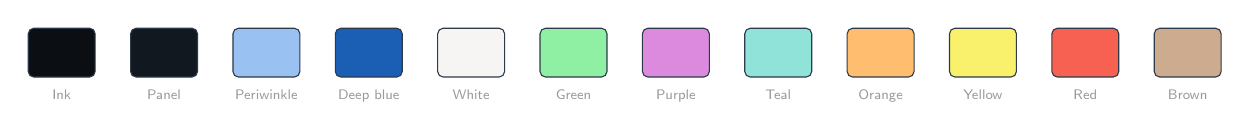
\begin{tikzpicture}[x=1cm,y=1cm]
  \foreach \c/\n [count=\i] in {ccblack/Ink,ccpanel/Panel,ccsky/Periwinkle,ccskyd/Deep blue,
      ccwhite/White,ccgreen/Green,ccpurple/Purple,ccteal/Teal,ccorange/Orange,ccyellow/Yellow,
      ccred/Red,ccbrown/Brown}{
    \fill[\c,draw=ccline,rounded corners=2pt] (\i*1.3-1.3,0) rectangle (\i*1.3-0.45,0.62);
    \node[font=\sffamily\tiny,text=ccgray,anchor=north,align=center] at (\i*1.3-0.875,-0.04) {\n};}
\end{tikzpicture}
\end{center}

\begin{center}\small
\begin{tabularx}{\linewidth}{@{}l l Y@{}}
\toprule
\textbf{Role} & \textbf{Hex} & \textbf{Use} \\
\midrule
Ink / background & \texttt{0B0F14} & window and deep panels \\
Periwinkle (primary) & \texttt{99C1F1} & brand, highlights, links on dark \\
Deep blue & \texttt{1A5FB4} & headings, links on white, active states \\
White & \texttt{F6F5F4} & text and surfaces on dark \\
Green & \texttt{8FF0A4} & success, voice-connected, ``add'' \\
Icon accents & GNOME hues & per-server colour code (blue, purple, green, teal, orange, yellow, red, brown) \\
\bottomrule
\end{tabularx}
\end{center}

\subsection{User interface}

The layout mirrors Discord so that nothing has to be learned, but the colours, logo and
assets are CyberCord's own. Two additions are unique to CyberCord: the voice panel shows
the room's topology level and who is hosting, and the member list groups people by their
network role (Hub, Standby, Keepers).

\clearpage
\begin{figure}[H]
\centering
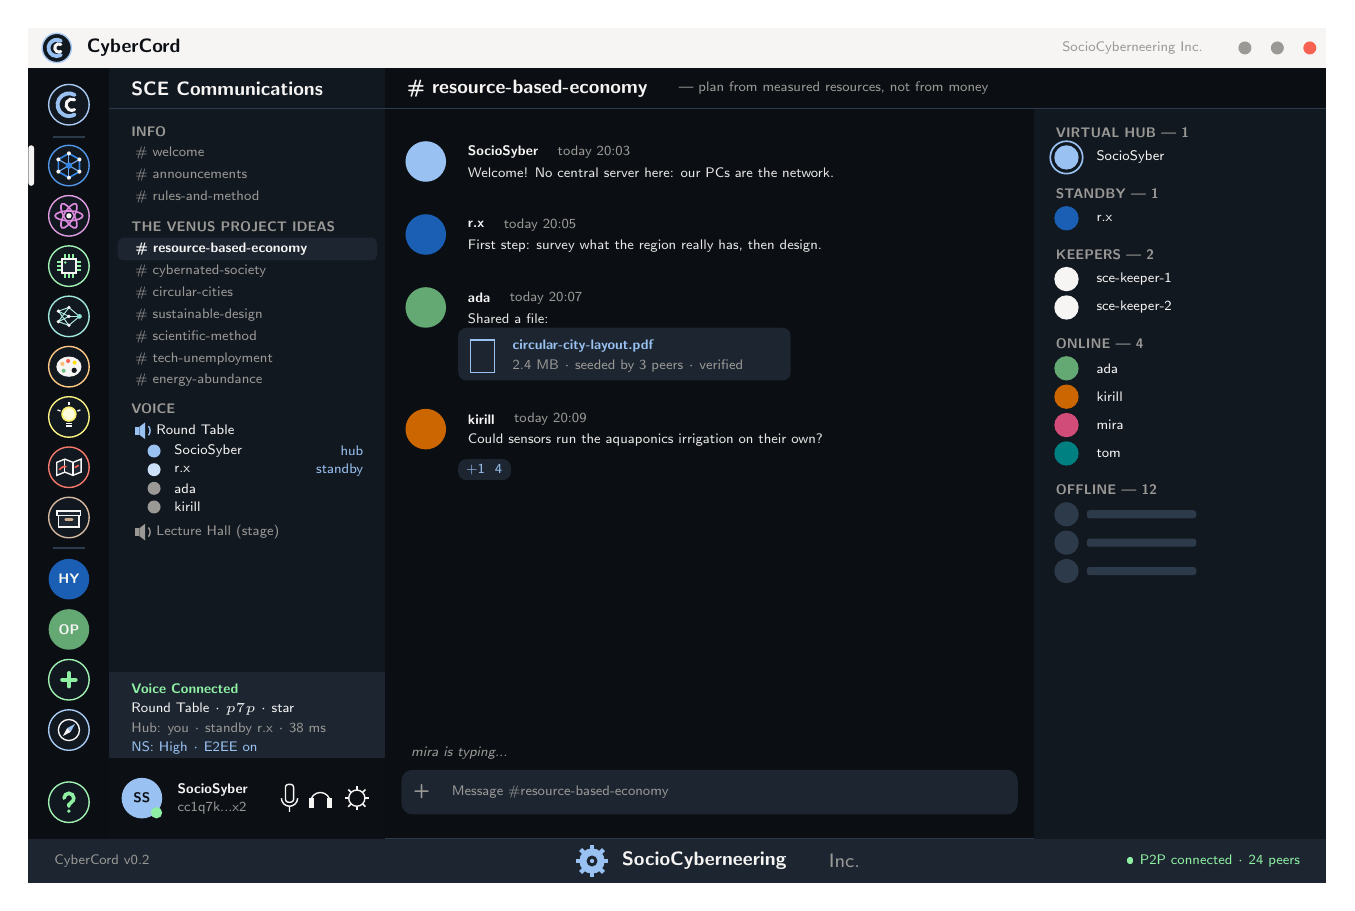
\begin{tikzpicture}[x=1.03cm,y=1.03cm,font=\sffamily]
  % window
  \fill[ccblack] (0,-0.55) rectangle (16,10);
  \fill[ccwhite] (0,9.5) rectangle (16,10);
  % ---- app bottom bar: logo + company ----
  \fill[ccpanel2] (0,-0.55) rectangle (16,0);
  \draw[ccline,line width=0.5pt] (0,0) -- (16,0);
  \begin{scope}[shift={(6.95,-0.275)},scale=0.2]
    \foreach \a in {0,45,...,315}{\fill[ccblue1,rotate=\a] (-0.13,0.74) rectangle (0.13,1.0);}
    \fill[ccblue1] (0,0) circle (0.78); \fill[ccpanel2] (0,0) circle (0.34); \fill[ccblue1] (0,0) circle (0.13);
  \end{scope}
  \node[anchor=west,text=ccwhite,font=\sffamily\scriptsize\bfseries] at (7.2,-0.275) {SocioCyberneering};
  \node[anchor=west,text=ccgray,font=\sffamily\scriptsize] at (9.75,-0.275) {Inc.};
  \node[anchor=west,text=ccgray,font=\sffamily\tiny] at (0.2,-0.275) {CyberCord v0.2};
  \node[anchor=east,text=ccgreen,font=\sffamily\tiny] at (15.8,-0.275) {\textbullet\ P2P connected $\cdot$ 24 peers};
  \pic[scale=0.36] at (0.35,9.75) {ic home};
  \node[anchor=west,font=\sffamily\scriptsize\bfseries,text=ccblack] at (0.6,9.75) {CyberCord};
  \node[anchor=east,font=\sffamily\tiny,text=ccgray] at (14.6,9.75) {SocioCyberneering Inc.};
  \foreach \x/\c in {15.0/ccgray,15.4/ccgray,15.8/ccred}{\fill[\c] (\x,9.75) circle (0.08);}
  % rail
  \fill[ccblack] (0,0) rectangle (1,9.5);
  {\colorlet{icacc}{ccblue1}\pic[scale=0.5] at (0.5,9.05) {ic home};}
  \draw[ccline,line width=0.8pt] (0.3,8.65) -- (0.7,8.65);
  \fill[ccwhite,rounded corners=1pt] (0,8.05) rectangle (0.07,8.55);
  {\colorlet{icacc}{ccblue3}\pic[scale=0.5] at (0.5,8.3) {ic sce};}
  {\colorlet{icacc}{ccpurple}\pic[scale=0.5] at (0.5,7.68) {ic atom};}
  {\colorlet{icacc}{ccgreen}\pic[scale=0.5] at (0.5,7.06) {ic pcb};}
  {\colorlet{icacc}{ccteal}\pic[scale=0.5] at (0.5,6.44) {ic ai};}
  {\colorlet{icacc}{ccorange}\pic[scale=0.5] at (0.5,5.82) {ic art};}
  {\colorlet{icacc}{ccyellow}\pic[scale=0.5] at (0.5,5.20) {ic idea};}
  {\colorlet{icacc}{ccred}\pic[scale=0.5] at (0.5,4.58) {ic gs};}
  {\colorlet{icacc}{ccbrown}\pic[scale=0.5] at (0.5,3.96) {ic archive};}
  \draw[ccline,line width=0.8pt] (0.3,3.58) -- (0.7,3.58);
  \fill[ccskyd] (0.5,3.2) circle (0.25); \node[text=ccwhite,font=\sffamily\tiny\bfseries] at (0.5,3.2) {HY};
  \fill[ccgreen!70!black] (0.5,2.58) circle (0.25); \node[text=ccwhite,font=\sffamily\tiny\bfseries] at (0.5,2.58) {OP};
  {\colorlet{icacc}{ccgreen}\pic[scale=0.5] at (0.5,1.96) {ic add};}
  {\colorlet{icacc}{ccblue1}\pic[scale=0.5] at (0.5,1.34) {ic explore};}
  {\colorlet{icacc}{ccgreen}\pic[scale=0.5] at (0.5,0.45) {ic help};}
  % channel sidebar
  \fill[ccpanel] (1,0) rectangle (4.4,9.5);
  \fill[ccpanel] (1,9.0) rectangle (4.4,9.5);
  \draw[ccline] (1,9.0) -- (4.4,9.0);
  \node[anchor=west,text=ccwhite,font=\sffamily\scriptsize\bfseries] at (1.15,9.25) {SCE Communications};
  \node[anchor=west,text=ccgray,font=\sffamily\tiny\bfseries] at (1.15,8.72) {INFO};
  \foreach \y/\t in {8.45/welcome,8.18/announcements,7.91/rules-and-method}{
    \node[anchor=west,text=ccgray,font=\sffamily\tiny] at (1.2,\y) {\#\ \t};}
  \node[anchor=west,text=ccgray,font=\sffamily\tiny\bfseries] at (1.15,7.55) {THE VENUS PROJECT IDEAS};
  \fill[ccpanel2,rounded corners=2pt] (1.1,7.13) rectangle (4.3,7.41);
  \node[anchor=west,text=ccwhite,font=\sffamily\tiny\bfseries] at (1.2,7.27) {\#\ resource-based-economy};
  \foreach \y/\t in {7.0/cybernated-society,6.73/circular-cities,6.46/sustainable-design,6.19/scientific-method,5.92/tech-unemployment,5.65/energy-abundance}{
    \node[anchor=west,text=ccgray,font=\sffamily\tiny] at (1.2,\y) {\#\ \t};}
  \node[anchor=west,text=ccgray,font=\sffamily\tiny\bfseries] at (1.15,5.3) {VOICE};
  \node[anchor=west,text=ccwhite,font=\sffamily\tiny] at (1.2,5.03) {\color{ccsky}\spk\ \color{ccwhite}Round Table};
  \foreach \y/\n/\r/\c in {4.78/SocioSyber/hub/ccsky,4.55/r.x/standby/ccsky!50,4.32/ada//ccgray,4.09/kirill//ccgray}{
    \fill[\c] (1.55,\y) circle (0.08);
    \node[anchor=west,text=ccwhite,font=\sffamily\tiny] at (1.68,\y) {\n};
    \node[anchor=east,text=ccsky,font=\sffamily\tiny] at (4.25,\y) {\r};}
  \node[anchor=west,text=ccgray,font=\sffamily\tiny] at (1.2,3.78) {\spk\ Lecture Hall (stage)};
  % voice connected panel
  \fill[ccpanel2] (1,1.0) rectangle (4.4,2.05);
  \node[anchor=west,text=ccgreen,font=\sffamily\tiny\bfseries] at (1.15,1.85) {Voice Connected};
  \node[anchor=west,text=ccwhite,font=\sffamily\tiny] at (1.15,1.6) {Round Table $\cdot$ $p7p$ $\cdot$ star};
  \node[anchor=west,text=ccgray,font=\sffamily\tiny] at (1.15,1.35) {Hub: you $\cdot$ standby r.x $\cdot$ 38 ms};
  \node[anchor=west,text=ccsky,font=\sffamily\tiny] at (1.15,1.12) {NS: High $\cdot$ E2EE on};
  % user panel
  \fill[ccblack!90!ccpanel] (1,0) rectangle (4.4,1.0);
  \fill[ccsky] (1.4,0.5) circle (0.25); \node[text=ccblack,font=\sffamily\tiny\bfseries] at (1.4,0.5) {SS};
  \fill[ccgreen] (1.58,0.32) circle (0.07);
  \node[anchor=west,text=ccwhite,font=\sffamily\tiny\bfseries] at (1.72,0.6) {SocioSyber};
  \node[anchor=west,text=ccgray,font=\sffamily\tiny] at (1.72,0.38) {cc1q7k...x2};
  % mic
  \draw[ccwhite,line width=0.5pt,rounded corners=1pt] (3.17,0.45) rectangle (3.27,0.67);
  \draw[ccwhite,line width=0.5pt] (3.12,0.5) arc (180:360:0.1) (3.22,0.4) -- (3.22,0.33);
  % headset
  \draw[ccwhite,line width=0.5pt] (3.48,0.45) arc (180:0:0.12);
  \fill[ccwhite] (3.46,0.38) rectangle (3.52,0.5); \fill[ccwhite] (3.68,0.38) rectangle (3.74,0.5);
  % gear
  \draw[ccwhite,line width=0.5pt] (4.05,0.5) circle (0.1);
  \foreach \a in {0,45,...,315}{\draw[ccwhite,line width=0.6pt] (4.05,0.5) ++(\a:0.1) -- ++(\a:0.05);}
  % chat area
  \draw[ccline] (4.4,9.0) -- (12.4,9.0);
  \node[anchor=west,text=ccwhite,font=\sffamily\scriptsize\bfseries] at (4.55,9.25) {\#\ resource-based-economy};
  \node[anchor=west,text=ccgray,font=\sffamily\tiny] at (7.9,9.25) {| plan from measured resources, not from money};
  % messages
  \foreach \y/\n/\c/\tm/\t in {
    8.35/SocioSyber/ccsky/20:03/{Welcome! No central server here: our PCs are the network.},
    7.45/r.x/ccskyd/20:05/{First step: survey what the region really has, then design.},
    6.55/ada/ccgreen!70!black/20:07/{Shared a file:},
    5.05/kirill/orange!80!black/20:09/{Could sensors run the aquaponics irrigation on their own?}}{
    \fill[\c] (4.9,\y) circle (0.25);
    \node[anchor=west,text=ccwhite,font=\sffamily\tiny\bfseries] (nm) at (5.3,\y+0.12) {\n};
    \node[anchor=west,text=ccgray,font=\sffamily\tiny] at (nm.east) {today \tm};
    \node[anchor=west,text=ccwhite!85!ccgray,font=\sffamily\tiny] at (5.3,\y-0.14) {\t};}
  % file card
  \fill[ccpanel2,rounded corners=3pt] (5.3,5.65) rectangle (9.4,6.3);
  \draw[ccsky,line width=0.5pt] (5.45,5.75) rectangle (5.75,6.15);
  \node[anchor=west,text=ccsky,font=\sffamily\tiny\bfseries] at (5.85,6.08) {circular-city-layout.pdf};
  \node[anchor=west,text=ccgray,font=\sffamily\tiny] at (5.85,5.83) {2.4 MB $\cdot$ seeded by 3 peers $\cdot$ verified};
  % reaction
  \fill[ccpanel2,rounded corners=3pt] (5.3,4.42) rectangle (5.95,4.68);
  \node[text=ccsky,font=\sffamily\tiny] at (5.62,4.55) {+1 \ 4};
  % typing + input
  \node[anchor=west,text=ccgray,font=\sffamily\tiny\itshape] at (4.6,1.05) {mira is typing...};
  \fill[ccpanel2,rounded corners=4pt] (4.6,0.3) rectangle (12.2,0.85);
  \node[text=ccgray,font=\sffamily\scriptsize\bfseries] at (4.85,0.575) {+};
  \node[anchor=west,text=ccgray,font=\sffamily\tiny] at (5.1,0.575) {Message \#resource-based-economy};
  % member list
  \fill[ccpanel] (12.4,0) rectangle (16,9.0);
  \draw[ccline] (12.4,9.0) -- (16,9.0);
  \node[anchor=west,text=ccgray,font=\sffamily\tiny\bfseries] at (12.55,8.7) {VIRTUAL HUB --- 1};
  \fill[ccsky] (12.8,8.4) circle (0.15); \draw[ccsky,line width=0.6pt] (12.8,8.4) circle (0.2);
  \node[anchor=west,text=ccwhite,font=\sffamily\tiny] at (13.05,8.4) {SocioSyber};
  \node[anchor=west,text=ccgray,font=\sffamily\tiny\bfseries] at (12.55,7.95) {STANDBY --- 1};
  \fill[ccskyd] (12.8,7.65) circle (0.15);
  \node[anchor=west,text=ccwhite,font=\sffamily\tiny] at (13.05,7.65) {r.x};
  \node[anchor=west,text=ccgray,font=\sffamily\tiny\bfseries] at (12.55,7.2) {KEEPERS --- 2};
  \foreach \y/\n in {6.9/sce-keeper-1,6.55/sce-keeper-2}{
    \fill[ccwhite] (12.8,\y) circle (0.15);
    \node[anchor=west,text=ccwhite,font=\sffamily\tiny] at (13.05,\y) {\n};}
  \node[anchor=west,text=ccgray,font=\sffamily\tiny\bfseries] at (12.55,6.1) {ONLINE --- 4};
  \foreach \y/\n/\c in {5.8/ada/ccgreen!70!black,5.45/kirill/orange!80!black,5.1/mira/purple!70,4.75/tom/teal}{
    \fill[\c] (12.8,\y) circle (0.15);
    \node[anchor=west,text=ccwhite,font=\sffamily\tiny] at (13.05,\y) {\n};}
  \node[anchor=west,text=ccgray,font=\sffamily\tiny\bfseries] at (12.55,4.3) {OFFLINE --- 12};
  \foreach \y in {4.0,3.65,3.3}{
    \fill[ccline] (12.8,\y) circle (0.15); \fill[ccline,rounded corners=1pt] (13.05,\y-0.05) rectangle (14.4,\y+0.05);}
\end{tikzpicture}
\caption{Main window wireframe: server rail (default servers, then the user's own
servers, add, explore, help), channel list, chat, member list grouped by network role,
voice panel showing topology level and hub.}
\label{fig:ui}
\end{figure}

% =====================================================================
\section{Default servers}
\label{sec:servers}
% =====================================================================

\subsection{How default servers exist without a central server}
Each default server is a \textbf{genesis manifest} compiled into the application and
signed by the SocioCyberneering root key (held offline, 2-of-3 threshold). Opening one
for the first time simply means: look up \texttt{H("guild"\,||\,id)} in the DHT and sync
from whoever is online --- other members or the SocioCyberneering Keepers running on the
\texttt{sociocyber.site} infrastructure. If the Keepers are down, members with replicas
still serve the history.

\subsection{Server rail order (user-friendly grouping)}
The rail is grouped so a newcomer sees, top to bottom: \emph{home}, the official hub,
the topic servers, then their own world. \emph{Help} is pinned at the bottom so it is
always in the same place.

\begin{center}
\small
\begin{tabularx}{\linewidth}{@{}c l Y@{}}
\toprule
\textbf{Icon} & \textbf{Server} & \textbf{Group / purpose} \\
\midrule
{\colorlet{icacc}{ccblue1}\icon{ic home}}    & Home & DMs, friends, mentions inbox \\
{\colorlet{icacc}{ccblue3}\icon{ic sce}}     & SocioCyberneering Communications & Official $\cdot$ ideas of The Venus Project \\
{\colorlet{icacc}{ccpurple}\icon{ic atom}}    & Atom-Generator & Science \& Engineering \\
{\colorlet{icacc}{ccgreen}\icon{ic pcb}}     & Automation & Science \& Engineering $\cdot$ PCB, electronics \\
{\colorlet{icacc}{ccteal}\icon{ic ai}}      & AI Design & Science \& Engineering $\cdot$ architecture, cities, Claude news \\
{\colorlet{icacc}{ccorange}\icon{ic art}}     & ART & Culture \\
{\colorlet{icacc}{ccyellow}\icon{ic idea}}    & Creativity & Culture \\
{\colorlet{icacc}{ccred}\icon{ic gs}}      & General-Semantics & Knowledge \\
{\colorlet{icacc}{ccbrown}\icon{ic archive}} & Archives & Knowledge $\cdot$ science papers \\
{\colorlet{icacc}{ccblue2}\icon{ic users}}   & User's servers & Servers you created or joined (folders allowed) \\
{\colorlet{icacc}{ccgreen}\icon{ic add}}     & Add a server & Create, join by invite link, or scan QR \\
{\colorlet{icacc}{ccblue1}\icon{ic explore}} & Explore & Public server directory from the DHT \\
{\colorlet{icacc}{ccgreen}\icon{ic help}}    & Help & Pinned at the bottom of the rail \\
\bottomrule
\end{tabularx}
\end{center}

\clearpage
\subsection{Channel layouts}

\begin{multicols}{2}
\raggedcolumns

\begin{serverbox}{\icon[0.42]{ic sce}\ SocioCyberneering Communications}
\cat{Info}
\ch{welcome}\\ \ch{announcements}\\ \ch{rules-and-method}
\cat{The Venus Project ideas (J. Fresco, before 2017)}
\ch{resource-based-economy}\\
\ch{cybernated-society}\\
\ch{circular-cities}\\
\ch{sustainable-design}\\
\ch{scientific-method}\\
\ch{tech-unemployment}\\
\ch{energy-abundance}\\
\ch{education-and-values}
\cat{Voice}
\vc{Round Table}\\ \vc{Lecture Hall} {\scriptsize(stage)}
\end{serverbox}

\begin{serverbox}{\icon[0.42]{ic atom}\ Atom-Generator}
\cat{Concept}
\ch{concept-overview}\\ \ch{feynman-plenty-of-room}\\ \ch{molecular-assembly}\\
\ch{energy-budget}\\ \ch{latex-docs}
\cat{Voice}
\vc{Lab}
\end{serverbox}

\begin{serverbox}{\icon[0.42]{ic pcb}\ Automation}
\cat{Hardware}
\ch{kicad-pcb}\\ \ch{power-electronics}\\ \ch{sensors-iot}\\ \ch{show-your-board}
\cat{Software}
\ch{embedded-rust}\\ \ch{orange-pi}\\ \ch{firmware}\\ \ch{hydroponics-automation}
\cat{Voice}
\vc{Workbench}
\end{serverbox}

\begin{serverbox}{\icon[0.42]{ic ai}\ AI Design}
\cat{Design}
\ch{architecture}\\ \ch{city-simulations}\\ \ch{generative-cad}\\ \ch{prompts-and-tools}
\cat{News}
\ch{claude-news} {\scriptsize(feed, read-only)}\\ \ch{claude-news-talk}
\cat{Voice}
\vc{Studio}
\end{serverbox}

\begin{serverbox}{\icon[0.42]{ic art}\ ART}
\ch{gallery}\\ \ch{digital-art}\\ \ch{generative-art}\\ \ch{wip}\\ \ch{critique}
\cat{Voice}
\vc{Atelier}
\end{serverbox}

\begin{serverbox}{\icon[0.42]{ic idea}\ Creativity}
\ch{ideas-board}\\ \ch{writing}\\ \ch{music}\\ \ch{weekly-challenge}\\ \ch{find-collaborators}
\cat{Voice}
\vc{Jam Room}
\end{serverbox}

\begin{serverbox}{\icon[0.42]{ic gs}\ General-Semantics}
\ch{map-is-not-the-territory}\\ \ch{extensional-devices}\\ \ch{structural-differential}\\
\ch{e-prime}\\ \ch{reading-club}
\cat{Voice}
\vc{Seminar}
\end{serverbox}

\begin{serverbox}{\icon[0.42]{ic archive}\ Archives}
\cat{Library}
\ch{physics}\\ \ch{mathematics}\\ \ch{computer-science}\\ \ch{electronics}\\
\ch{biology-and-agro}\\ \ch{geology-and-materials}
\cat{Service}
\ch{paper-requests}\\ \ch{library-rules}
\end{serverbox}

\begin{serverbox}{\icon[0.42]{ic help}\ Help}
\ch{start-here}\\ \ch{faq}\\ \ch{bug-reports}\\ \ch{feature-requests}\\ \ch{protocol-dev}
\cat{Voice}
\vc{Support Desk}
\end{serverbox}

\end{multicols}

\begin{note}[Server-specific notes]
\begin{itemize}[leftmargin=1.2em]
  \item \textbf{SocioCyberneering Communications} discusses the published ideas of Jacque
        Fresco and The Venus Project up to 2017. State in \ch{welcome} that the server is
        a discussion community and not affiliated with The Venus Project organisation.
  \item \textbf{\#claude-news} is fed by a bot peer running on a Keeper that bridges the public
        Anthropic news feed into a read-only channel; discussion happens in
        \ch{claude-news-talk}.
  \item \textbf{Archives} keeps a \emph{library view}: each paper is a blob with title, authors,
        DOI and licence. Policy: open-access, preprint or author-uploaded papers only;
        moderators remove infringing items with a takedown event that honest peers obey.
  \item \textbf{User's servers} supports folders exactly like Discord; new servers get a
        template picker (Community, Project, Study group, Family).
\end{itemize}
\end{note}

\needspace{12\baselineskip}
% =====================================================================
\section{Security and privacy}
\label{sec:threats}
% =====================================================================

\begin{longtable}{@{}p{0.25\linewidth}p{0.68\linewidth}@{}}
\toprule
\textbf{Threat} & \textbf{Mitigation} \\
\midrule
\endhead
Forged messages & Ed25519 signatures on every event; IDs are hashes over parents. \\
Malicious hub (drops, delays) & Receipt digests compared via standby; local veto and re-election; hub never sees plaintext of private rooms. \\
Sybil accounts, spam & Invite tokens or proof-of-work to join; per-author rate limits enforced by every peer; moderator bans as events. \\
DHT eclipse attack & Multiple disjoint lookups, peer diversity by IP prefix, signed seed list, cached trusted peers. \\
IP address exposure & \textbf{Shielded mode}: no direct links, never hub, all traffic through relays or the \textbf{CyberVPN} tunnel. \\
Metadata to hub & Hub sees who is in a room and when they speak (audio level), not content. Shielded mode hides IP. \\
Lost keys & 24-word recovery phrase; device certificates; guild owner threshold 2-of-3. \\
Malicious files & No auto-open or execution; previews rendered in a sandbox; per-guild size limits; hashes shown. \\
Illegal content & Guild moderation, takedown events, Archives open-access policy; Keepers obey takedowns. \\
Deletion requests & Delete events honoured by all honest clients; limitation stated openly to users. \\
\bottomrule
\end{longtable}

\needspace{12\baselineskip}
% =====================================================================
\section{Roadmap}
% =====================================================================

\begin{center}
\small
\begin{tabularx}{\linewidth}{@{}l l Y@{}}
\toprule
\textbf{Phase} & \textbf{Name} & \textbf{Deliverable} \\
\midrule
M0 & Concept & This document; protocol name and parameters agreed. \\
M1 & Wire \& identity & \texttt{cc-proto}, \texttt{cc-net}; two CLI peers chat over QUIC with mDNS + DHT + hole punching. \\
M2 & History & Event DAG, auth rules, SQLite store, set reconciliation, guild manifests, roles, invites. \\
M3 & Hub \& voice MVP & Score, election, lease/failover; Opus voice with RNNoise; mesh $\leftrightarrow$ star switching. \\
M4 & Desktop app & Tauri UI (Discord-like) on Windows and GNU/Linux; default servers; installers. \\
M5 & Files \& Keepers & Blob swarming, Keeper daemon (OpenRC/runit/s6/dinit/systemd, Windows service), mailboxes, QR invites. \\
M6 & Privacy & MLS for DMs/private channels, SFrame for media, Shielded mode with CyberVPN. \\
M7 & Media+ & Video, screen share, stage channels, cascaded hubs, bot SDK. \\
\bottomrule
\end{tabularx}
\end{center}

% =====================================================================
\section{Open questions}
% =====================================================================
\begin{enumerate}
  \item \textbf{libp2p or iroh?} libp2p lets \emph{any} peer relay (fits ``no central
        server'' best); iroh is simpler and fast but its default relays are operated
        servers (can be self-hosted). Decide with an M1 prototype.
  \item \textbf{Score weights.} The values in Eq.~\eqref{eq:score} are a starting point; tune
        with real measurements from test rooms.
  \item \textbf{Large public servers.} How far can pure peer moderation scale before
        trust/reputation systems are needed?
  \item \textbf{Mobile clients} (later): never eligible as hub; push notifications without a
        central service are an unsolved problem worth its own document.
\end{enumerate}

\bigskip
\begin{center}
\small\color{ccgray}
CyberCord reproduces the familiar layout and feature set of popular chat applications
with its own name, logo, colours and artwork; it is not affiliated with Discord Inc.\\[4pt]
\textcopyright\ 2026 SocioCyberneering Inc. $\cdot$ sociocyber.site
\end{center}

\clearpage
% =====================================================================
\appendix
\section{Core Rust types (draft)}
% =====================================================================

\begin{lstlisting}[language=Rust]
/// 32-byte BLAKE3 hash of an Ed25519 public key.
pub struct UserId(pub [u8; 32]);
pub struct EventId(pub [u8; 32]);
pub struct GuildId(pub [u8; 32]);
pub struct ChannelId(pub [u8; 16]);

/// Every piece of guild data is a signed event in a DAG.
pub struct Event {
    pub version: u8,
    pub guild: GuildId,
    pub channel: Option<ChannelId>,
    pub author: UserId,
    pub device: [u8; 32],          // device public key (certified by author)
    pub parents: Vec<EventId>,     // 1..=4 latest heads seen by author
    pub lamport: u64,
    pub wall_time_ms: i64,         // advisory only
    pub kind: EventKind,
    pub sig: [u8; 64],             // Ed25519 over all fields above
}

pub enum EventKind {
    Genesis { name: String, owner_keys: Vec<[u8; 32]>, threshold: u8 },
    ChannelCreate { id: ChannelId, name: String, kind: ChannelKind },
    Message { body: String, reply_to: Option<EventId>, blobs: Vec<BlobRef> },
    Edit { target: EventId, body: String },
    Delete { target: EventId },
    Reaction { target: EventId, emoji: String, add: bool },
    RoleSet { user: UserId, roles: Vec<u16> },
    Ban { user: UserId, reason: Option<String> },
    Mls(Vec<u8>),                  // opaque MLS ciphertext for private channels
}

pub enum ChannelKind { Text, Voice, Stage, Feed }

pub struct BlobRef { pub root: [u8; 32], pub size: u64, pub mime: String,
                     pub key: Option<[u8; 32]> }

/// Gossiped every 5 s by each peer in a room.
pub struct HubScore {
    pub peer: UserId,
    pub channel: ChannelId,
    pub uplink_kbps: u32,
    pub median_rtt_ms: u16,
    pub nat: NatClass,
    pub online_secs: u32,
    pub on_ac_power: bool,
    pub load: f32,                 // share of capacity already used, 0..1
    pub never_host: bool,
    pub sig: [u8; 64],
}

pub enum NatClass { Public, FullCone, Restricted, Symmetric }

pub struct Lease {
    pub channel: ChannelId,
    pub epoch: u64,
    pub hub: UserId,
    pub standby: UserId,
    pub expires_ms: i64,
    pub sig: [u8; 64],             // signed by hub
}

/// Header of a voice datagram (payload = SFrame(Opus)).
pub struct MediaHeader {
    pub room: u16,                 // short id negotiated on VOICE_JOIN
    pub stream: u32,
    pub seq: u16,
    pub ts: u32,                   // 48 kHz sample clock
    pub level: u8,                 // audio level for loudest-speaker selection
    pub flags: u8,                 // FEC, DTX, keyframe...
}
\end{lstlisting}

\needspace{18\baselineskip}
\begin{lstlisting}[language=Rust]
/// Effective hub score: Eq. (4) times (1 - load). Returns 0.0 when vetoed.
pub fn hub_score(s: &HubScore) -> f32 {
    if s.never_host { return 0.0; }
    let b = ((1.0 + s.uplink_kbps as f32 / 1000.0).ln() / 101f32.ln()).min(1.0);
    let c = 1.0 - (s.median_rtt_ms.min(300) as f32 / 300.0);
    let r = match s.nat {
        NatClass::Public => 1.0, NatClass::FullCone => 0.8,
        NatClass::Restricted => 0.5, NatClass::Symmetric => 0.1,
    };
    let t = (s.online_secs as f32 / 1800.0).min(1.0);
    let p = if s.on_ac_power { 1.0 } else { 0.3 };
    let raw = 0.35 * b + 0.25 * c + 0.20 * r + 0.10 * t + 0.10 * p;
    raw * (1.0 - s.load.clamp(0.0, 1.0))
}
\end{lstlisting}


\end{document}
